% Copyright © 2013 Martin Ueding <dev@martin-ueding.de>

% Copyright © 2012-2013 Martin Ueding <dev@martin-ueding.de>

% This is my general purpose LaTeX header file for writing German documents.
% Ideally, you include this using a simple ``% Copyright © 2012-2013 Martin Ueding <dev@martin-ueding.de>

% This is my general purpose LaTeX header file for writing German documents.
% Ideally, you include this using a simple ``% Copyright © 2012-2013 Martin Ueding <dev@martin-ueding.de>

% This is my general purpose LaTeX header file for writing German documents.
% Ideally, you include this using a simple ``\input{header.tex}`` in your main
% document and start with ``\title`` and ``\begin{document}`` afterwards.

% If you need to add additional packages, I recommend not doing this in this
% file, but in your main document. That way, you can just drop in a new
% ``header.tex`` and get all the new commands without having to merge manually.

% Since this file encorporates a CC-BY-SA fragment, this whole files is
% licensed under the CC-BY-SA license.

\documentclass[11pt, ngerman, fleqn, DIV=15, headinclude, BCOR=2cm]{scrartcl}

\usepackage{graphicx}

% Environment to quote the problem. Currently, this is just a new name for the
% quote environment.
\newenvironment{problem}{\begin{quote}\textsf{\textbf{Aufgabenstellung:}}\quad}{\end{quote}}

\setkomafont{caption}{\sf}
\setkomafont{captionlabel}{\usekomafont{caption}}

%%%%%%%%%%%%%%%%%%%%%%%%%%%%%%%%%%%%%%%%%%%%%%%%%%%%%%%%%%%%%%%%%%%%%%%%%%%%%%%
%                                Locale, date                                 %
%%%%%%%%%%%%%%%%%%%%%%%%%%%%%%%%%%%%%%%%%%%%%%%%%%%%%%%%%%%%%%%%%%%%%%%%%%%%%%%

\usepackage{babel}
\usepackage[iso]{isodate}

%%%%%%%%%%%%%%%%%%%%%%%%%%%%%%%%%%%%%%%%%%%%%%%%%%%%%%%%%%%%%%%%%%%%%%%%%%%%%%%
%                          Margins and other spacing                          %
%%%%%%%%%%%%%%%%%%%%%%%%%%%%%%%%%%%%%%%%%%%%%%%%%%%%%%%%%%%%%%%%%%%%%%%%%%%%%%%

\usepackage[parfill]{parskip}
\usepackage{setspace}
\usepackage[activate]{microtype}

\setlength{\columnsep}{2cm}

%%%%%%%%%%%%%%%%%%%%%%%%%%%%%%%%%%%%%%%%%%%%%%%%%%%%%%%%%%%%%%%%%%%%%%%%%%%%%%%
%                                    Color                                    %
%%%%%%%%%%%%%%%%%%%%%%%%%%%%%%%%%%%%%%%%%%%%%%%%%%%%%%%%%%%%%%%%%%%%%%%%%%%%%%%

\usepackage[usenames, dvipsnames]{xcolor}

\colorlet{darkred}{red!70!black}
\colorlet{darkblue}{blue!70!black}
\colorlet{darkgreen}{green!40!black}

%%%%%%%%%%%%%%%%%%%%%%%%%%%%%%%%%%%%%%%%%%%%%%%%%%%%%%%%%%%%%%%%%%%%%%%%%%%%%%%
%                         Font and font like settings                         %
%%%%%%%%%%%%%%%%%%%%%%%%%%%%%%%%%%%%%%%%%%%%%%%%%%%%%%%%%%%%%%%%%%%%%%%%%%%%%%%

% This replaces all fonts with Bitstream Charter, Bitstream Vera Sans and
% Bitstream Vera Mono. Math will be rendered in Charter.
\usepackage[charter, greekuppercase=italicized]{mathdesign}
\usepackage{beramono}
\usepackage{berasans}

% Bold, sans-serif tensors. This fragment is taken from “egreg” from
% http://tex.stackexchange.com/a/82747/8945 and licensed under `CC-BY-SA
% <https://creativecommons.org/licenses/by-sa/3.0/>`_.
\usepackage{bm}
\DeclareMathAlphabet{\mathsfit}{\encodingdefault}{\sfdefault}{m}{sl}
\SetMathAlphabet{\mathsfit}{bold}{\encodingdefault}{\sfdefault}{bx}{sl}
\newcommand{\tens}[1]{\bm{\mathsfit{#1}}}

% Bold vectors.
\renewcommand{\vec}[1]{\boldsymbol{#1}}

%%%%%%%%%%%%%%%%%%%%%%%%%%%%%%%%%%%%%%%%%%%%%%%%%%%%%%%%%%%%%%%%%%%%%%%%%%%%%%%
%                               Input encoding                                %
%%%%%%%%%%%%%%%%%%%%%%%%%%%%%%%%%%%%%%%%%%%%%%%%%%%%%%%%%%%%%%%%%%%%%%%%%%%%%%%

\usepackage[T1]{fontenc}
\usepackage[utf8]{inputenc}

%%%%%%%%%%%%%%%%%%%%%%%%%%%%%%%%%%%%%%%%%%%%%%%%%%%%%%%%%%%%%%%%%%%%%%%%%%%%%%%
%                         Hyperrefs and PDF metadata                          %
%%%%%%%%%%%%%%%%%%%%%%%%%%%%%%%%%%%%%%%%%%%%%%%%%%%%%%%%%%%%%%%%%%%%%%%%%%%%%%%

\usepackage{hyperref}
\usepackage{lastpage}

% This sets the author in the properties of the PDF as well. If you want to
% change it, just override it with another ``\hypersetup`` call.
\hypersetup{
	breaklinks=false,
	citecolor=darkgreen,
	colorlinks=true,
	linkcolor=darkblue,
	menucolor=black,
	pdfauthor={Martin Ueding},
	urlcolor=darkblue,
}

%%%%%%%%%%%%%%%%%%%%%%%%%%%%%%%%%%%%%%%%%%%%%%%%%%%%%%%%%%%%%%%%%%%%%%%%%%%%%%%
%                               Math Operators                                %
%%%%%%%%%%%%%%%%%%%%%%%%%%%%%%%%%%%%%%%%%%%%%%%%%%%%%%%%%%%%%%%%%%%%%%%%%%%%%%%

% AMS environments like ``align`` and theorems like ``proof``.
\usepackage{amsmath}
\usepackage{amsthm}

% Common math constructs like partial derivatives.
\usepackage{commath}

% Physical units.
\usepackage[output-decimal-marker={,}]{siunitx}

% Since I use mathdesign with italic uppercase greek characters, the Ohm unit will be displayed with an italic Ω by default. Units have to be roman, so this forces it the right way.
\DeclareSIUnit{\ohm}{$\Omegaup$}
\DeclareSIUnit{\division}{DIV}
\DeclareSIUnit{\voltss}{$\mathrm{V_{SS}}$}

% Word like operators.
\DeclareMathOperator{\acosh}{arcosh}
\DeclareMathOperator{\arcosh}{arcosh}
\DeclareMathOperator{\arcsinh}{arsinh}
\DeclareMathOperator{\arsinh}{arsinh}
\DeclareMathOperator{\asinh}{arsinh}
\DeclareMathOperator{\card}{card}
\DeclareMathOperator{\csch}{cshs}
\DeclareMathOperator{\diam}{diam}
\DeclareMathOperator{\sech}{sech}
\renewcommand{\Im}{\mathop{{}\mathrm{Im}}\nolimits}
\renewcommand{\Re}{\mathop{{}\mathrm{Re}}\nolimits}

% Fourier transform.
\DeclareMathOperator{\fourier}{\ensuremath{\mathcal{F}}}

% Roman versions of “e” and “i” to serve as Euler's number and the imaginary
% constant.
\newcommand{\ee}{\eup}
\newcommand{\eup}{\mathrm e}
\newcommand{\ii}{\iup}
\newcommand{\iup}{\mathrm i}

% Symbols for the various mathematical fields (natural numbers, integers,
% rational numbers, real numbers, complex numbers).
\newcommand{\C}{\ensuremath{\mathbb C}}
\newcommand{\N}{\ensuremath{\mathbb N}}
\newcommand{\Q}{\ensuremath{\mathbb Q}}
\newcommand{\R}{\ensuremath{\mathbb R}}
\newcommand{\Z}{\ensuremath{\mathbb Z}}

% Shape like operators.
\DeclareMathOperator{\dalambert}{\Box}
\DeclareMathOperator{\laplace}{\bigtriangleup}
\newcommand{\curl}{\vnabla \times}
\newcommand{\divergence}[1]{\inner{\vnabla}{#1}}
\newcommand{\vnabla}{\vec \nabla}

\newcommand{\half}{\frac 12}

% Unit vector (German „Einheitsvektor“).
\newcommand{\ev}{\hat{\vec e}}

% Scientific notation for large numbers.
\newcommand{\e}[1]{\cdot 10^{#1}}

% Mathematician's notation for the inner (scalar, dot) product.
\newcommand{\bracket}[1]{\left\langle #1 \right\rangle}
\newcommand{\inner}[2]{\bracket{#1, #2}}

% Placeholders.
\newcommand{\emesswert}{\del{\messwert \pm \messwert}}
\newcommand{\fehlt}{\textcolor{darkred}{Hier fehlen noch Inhalte.}}
\newcommand{\messwert}{\textcolor{blue}{\square}}
\newcommand{\punkte}{\phantom{xxxxx}}
\newcommand{\punktevon}[1]{\begin{flushright}/ #1\end{flushright}}

% Separator for equations on a single line.
\newcommand{\eqnsep}{,\quad}

% Quantum Mechanics
\usepackage{braket}

%%%%%%%%%%%%%%%%%%%%%%%%%%%%%%%%%%%%%%%%%%%%%%%%%%%%%%%%%%%%%%%%%%%%%%%%%%%%%%%
%                                  Headings                                   %
%%%%%%%%%%%%%%%%%%%%%%%%%%%%%%%%%%%%%%%%%%%%%%%%%%%%%%%%%%%%%%%%%%%%%%%%%%%%%%%

% This will set fancy headings to the top of the page. The page number will be
% accompanied by the total number of pages. That way, you will know if any page
% is missing.
%
% If you do not want this for your document, you can just use
% ``\pagestyle{plain}``.

\usepackage{scrpage2}

\pagestyle{scrheadings}
\automark{section}
\cfoot{\footnotesize{Seite \thepage\ / \pageref{LastPage}}}
\chead{}
\ihead{}
\ohead{\rightmark}
\setheadsepline{.4pt}

%%%%%%%%%%%%%%%%%%%%%%%%%%%%%%%%%%%%%%%%%%%%%%%%%%%%%%%%%%%%%%%%%%%%%%%%%%%%%%%
%                            Bibliography (BibTeX)                            %
%%%%%%%%%%%%%%%%%%%%%%%%%%%%%%%%%%%%%%%%%%%%%%%%%%%%%%%%%%%%%%%%%%%%%%%%%%%%%%%

\newcommand{\bibliographyfile}{../../../zentrale_BibTeX/Central}
\bibliographystyle{apalike2}

%%%%%%%%%%%%%%%%%%%%%%%%%%%%%%%%%%%%%%%%%%%%%%%%%%%%%%%%%%%%%%%%%%%%%%%%%%%%%%%
%                                Abbreviations                                %
%%%%%%%%%%%%%%%%%%%%%%%%%%%%%%%%%%%%%%%%%%%%%%%%%%%%%%%%%%%%%%%%%%%%%%%%%%%%%%%

\newcommand{\dhabk}{\mbox{d.\,h.}}

%%%%%%%%%%%%%%%%%%%%%%%%%%%%%%%%%%%%%%%%%%%%%%%%%%%%%%%%%%%%%%%%%%%%%%%%%%%%%%%
%                                  Licences                                   %
%%%%%%%%%%%%%%%%%%%%%%%%%%%%%%%%%%%%%%%%%%%%%%%%%%%%%%%%%%%%%%%%%%%%%%%%%%%%%%%

\usepackage{ccicons}

\newcommand{\ccbysadetext}{%
	\begin{small}
		Dieses Werk bzw. Inhalt steht unter einer
		\href{http://creativecommons.org/licenses/by-sa/3.0/deed.de}{%
			Creative Commons Namensnennung - Weitergabe unter gleichen
		Bedingungen 3.0 Unported Lizenz}.
	\end{small}
}

\newcommand{\ccbysadetitle}{%
	Lizenz: \href{http://creativecommons.org/licenses/by-sa/3.0/deed.de}
	{CC-BY-SA 3.0 \ccbysa}
}
`` in your main
% document and start with ``\title`` and ``\begin{document}`` afterwards.

% If you need to add additional packages, I recommend not doing this in this
% file, but in your main document. That way, you can just drop in a new
% ``header.tex`` and get all the new commands without having to merge manually.

% Since this file encorporates a CC-BY-SA fragment, this whole files is
% licensed under the CC-BY-SA license.

\documentclass[11pt, ngerman, fleqn, DIV=15, headinclude, BCOR=2cm]{scrartcl}

\usepackage{graphicx}

% Environment to quote the problem. Currently, this is just a new name for the
% quote environment.
\newenvironment{problem}{\begin{quote}\textsf{\textbf{Aufgabenstellung:}}\quad}{\end{quote}}

\setkomafont{caption}{\sf}
\setkomafont{captionlabel}{\usekomafont{caption}}

%%%%%%%%%%%%%%%%%%%%%%%%%%%%%%%%%%%%%%%%%%%%%%%%%%%%%%%%%%%%%%%%%%%%%%%%%%%%%%%
%                                Locale, date                                 %
%%%%%%%%%%%%%%%%%%%%%%%%%%%%%%%%%%%%%%%%%%%%%%%%%%%%%%%%%%%%%%%%%%%%%%%%%%%%%%%

\usepackage{babel}
\usepackage[iso]{isodate}

%%%%%%%%%%%%%%%%%%%%%%%%%%%%%%%%%%%%%%%%%%%%%%%%%%%%%%%%%%%%%%%%%%%%%%%%%%%%%%%
%                          Margins and other spacing                          %
%%%%%%%%%%%%%%%%%%%%%%%%%%%%%%%%%%%%%%%%%%%%%%%%%%%%%%%%%%%%%%%%%%%%%%%%%%%%%%%

\usepackage[parfill]{parskip}
\usepackage{setspace}
\usepackage[activate]{microtype}

\setlength{\columnsep}{2cm}

%%%%%%%%%%%%%%%%%%%%%%%%%%%%%%%%%%%%%%%%%%%%%%%%%%%%%%%%%%%%%%%%%%%%%%%%%%%%%%%
%                                    Color                                    %
%%%%%%%%%%%%%%%%%%%%%%%%%%%%%%%%%%%%%%%%%%%%%%%%%%%%%%%%%%%%%%%%%%%%%%%%%%%%%%%

\usepackage[usenames, dvipsnames]{xcolor}

\colorlet{darkred}{red!70!black}
\colorlet{darkblue}{blue!70!black}
\colorlet{darkgreen}{green!40!black}

%%%%%%%%%%%%%%%%%%%%%%%%%%%%%%%%%%%%%%%%%%%%%%%%%%%%%%%%%%%%%%%%%%%%%%%%%%%%%%%
%                         Font and font like settings                         %
%%%%%%%%%%%%%%%%%%%%%%%%%%%%%%%%%%%%%%%%%%%%%%%%%%%%%%%%%%%%%%%%%%%%%%%%%%%%%%%

% This replaces all fonts with Bitstream Charter, Bitstream Vera Sans and
% Bitstream Vera Mono. Math will be rendered in Charter.
\usepackage[charter, greekuppercase=italicized]{mathdesign}
\usepackage{beramono}
\usepackage{berasans}

% Bold, sans-serif tensors. This fragment is taken from “egreg” from
% http://tex.stackexchange.com/a/82747/8945 and licensed under `CC-BY-SA
% <https://creativecommons.org/licenses/by-sa/3.0/>`_.
\usepackage{bm}
\DeclareMathAlphabet{\mathsfit}{\encodingdefault}{\sfdefault}{m}{sl}
\SetMathAlphabet{\mathsfit}{bold}{\encodingdefault}{\sfdefault}{bx}{sl}
\newcommand{\tens}[1]{\bm{\mathsfit{#1}}}

% Bold vectors.
\renewcommand{\vec}[1]{\boldsymbol{#1}}

%%%%%%%%%%%%%%%%%%%%%%%%%%%%%%%%%%%%%%%%%%%%%%%%%%%%%%%%%%%%%%%%%%%%%%%%%%%%%%%
%                               Input encoding                                %
%%%%%%%%%%%%%%%%%%%%%%%%%%%%%%%%%%%%%%%%%%%%%%%%%%%%%%%%%%%%%%%%%%%%%%%%%%%%%%%

\usepackage[T1]{fontenc}
\usepackage[utf8]{inputenc}

%%%%%%%%%%%%%%%%%%%%%%%%%%%%%%%%%%%%%%%%%%%%%%%%%%%%%%%%%%%%%%%%%%%%%%%%%%%%%%%
%                         Hyperrefs and PDF metadata                          %
%%%%%%%%%%%%%%%%%%%%%%%%%%%%%%%%%%%%%%%%%%%%%%%%%%%%%%%%%%%%%%%%%%%%%%%%%%%%%%%

\usepackage{hyperref}
\usepackage{lastpage}

% This sets the author in the properties of the PDF as well. If you want to
% change it, just override it with another ``\hypersetup`` call.
\hypersetup{
	breaklinks=false,
	citecolor=darkgreen,
	colorlinks=true,
	linkcolor=darkblue,
	menucolor=black,
	pdfauthor={Martin Ueding},
	urlcolor=darkblue,
}

%%%%%%%%%%%%%%%%%%%%%%%%%%%%%%%%%%%%%%%%%%%%%%%%%%%%%%%%%%%%%%%%%%%%%%%%%%%%%%%
%                               Math Operators                                %
%%%%%%%%%%%%%%%%%%%%%%%%%%%%%%%%%%%%%%%%%%%%%%%%%%%%%%%%%%%%%%%%%%%%%%%%%%%%%%%

% AMS environments like ``align`` and theorems like ``proof``.
\usepackage{amsmath}
\usepackage{amsthm}

% Common math constructs like partial derivatives.
\usepackage{commath}

% Physical units.
\usepackage[output-decimal-marker={,}]{siunitx}

% Since I use mathdesign with italic uppercase greek characters, the Ohm unit will be displayed with an italic Ω by default. Units have to be roman, so this forces it the right way.
\DeclareSIUnit{\ohm}{$\Omegaup$}
\DeclareSIUnit{\division}{DIV}
\DeclareSIUnit{\voltss}{$\mathrm{V_{SS}}$}

% Word like operators.
\DeclareMathOperator{\acosh}{arcosh}
\DeclareMathOperator{\arcosh}{arcosh}
\DeclareMathOperator{\arcsinh}{arsinh}
\DeclareMathOperator{\arsinh}{arsinh}
\DeclareMathOperator{\asinh}{arsinh}
\DeclareMathOperator{\card}{card}
\DeclareMathOperator{\csch}{cshs}
\DeclareMathOperator{\diam}{diam}
\DeclareMathOperator{\sech}{sech}
\renewcommand{\Im}{\mathop{{}\mathrm{Im}}\nolimits}
\renewcommand{\Re}{\mathop{{}\mathrm{Re}}\nolimits}

% Fourier transform.
\DeclareMathOperator{\fourier}{\ensuremath{\mathcal{F}}}

% Roman versions of “e” and “i” to serve as Euler's number and the imaginary
% constant.
\newcommand{\ee}{\eup}
\newcommand{\eup}{\mathrm e}
\newcommand{\ii}{\iup}
\newcommand{\iup}{\mathrm i}

% Symbols for the various mathematical fields (natural numbers, integers,
% rational numbers, real numbers, complex numbers).
\newcommand{\C}{\ensuremath{\mathbb C}}
\newcommand{\N}{\ensuremath{\mathbb N}}
\newcommand{\Q}{\ensuremath{\mathbb Q}}
\newcommand{\R}{\ensuremath{\mathbb R}}
\newcommand{\Z}{\ensuremath{\mathbb Z}}

% Shape like operators.
\DeclareMathOperator{\dalambert}{\Box}
\DeclareMathOperator{\laplace}{\bigtriangleup}
\newcommand{\curl}{\vnabla \times}
\newcommand{\divergence}[1]{\inner{\vnabla}{#1}}
\newcommand{\vnabla}{\vec \nabla}

\newcommand{\half}{\frac 12}

% Unit vector (German „Einheitsvektor“).
\newcommand{\ev}{\hat{\vec e}}

% Scientific notation for large numbers.
\newcommand{\e}[1]{\cdot 10^{#1}}

% Mathematician's notation for the inner (scalar, dot) product.
\newcommand{\bracket}[1]{\left\langle #1 \right\rangle}
\newcommand{\inner}[2]{\bracket{#1, #2}}

% Placeholders.
\newcommand{\emesswert}{\del{\messwert \pm \messwert}}
\newcommand{\fehlt}{\textcolor{darkred}{Hier fehlen noch Inhalte.}}
\newcommand{\messwert}{\textcolor{blue}{\square}}
\newcommand{\punkte}{\phantom{xxxxx}}
\newcommand{\punktevon}[1]{\begin{flushright}/ #1\end{flushright}}

% Separator for equations on a single line.
\newcommand{\eqnsep}{,\quad}

% Quantum Mechanics
\usepackage{braket}

%%%%%%%%%%%%%%%%%%%%%%%%%%%%%%%%%%%%%%%%%%%%%%%%%%%%%%%%%%%%%%%%%%%%%%%%%%%%%%%
%                                  Headings                                   %
%%%%%%%%%%%%%%%%%%%%%%%%%%%%%%%%%%%%%%%%%%%%%%%%%%%%%%%%%%%%%%%%%%%%%%%%%%%%%%%

% This will set fancy headings to the top of the page. The page number will be
% accompanied by the total number of pages. That way, you will know if any page
% is missing.
%
% If you do not want this for your document, you can just use
% ``\pagestyle{plain}``.

\usepackage{scrpage2}

\pagestyle{scrheadings}
\automark{section}
\cfoot{\footnotesize{Seite \thepage\ / \pageref{LastPage}}}
\chead{}
\ihead{}
\ohead{\rightmark}
\setheadsepline{.4pt}

%%%%%%%%%%%%%%%%%%%%%%%%%%%%%%%%%%%%%%%%%%%%%%%%%%%%%%%%%%%%%%%%%%%%%%%%%%%%%%%
%                            Bibliography (BibTeX)                            %
%%%%%%%%%%%%%%%%%%%%%%%%%%%%%%%%%%%%%%%%%%%%%%%%%%%%%%%%%%%%%%%%%%%%%%%%%%%%%%%

\newcommand{\bibliographyfile}{../../../zentrale_BibTeX/Central}
\bibliographystyle{apalike2}

%%%%%%%%%%%%%%%%%%%%%%%%%%%%%%%%%%%%%%%%%%%%%%%%%%%%%%%%%%%%%%%%%%%%%%%%%%%%%%%
%                                Abbreviations                                %
%%%%%%%%%%%%%%%%%%%%%%%%%%%%%%%%%%%%%%%%%%%%%%%%%%%%%%%%%%%%%%%%%%%%%%%%%%%%%%%

\newcommand{\dhabk}{\mbox{d.\,h.}}

%%%%%%%%%%%%%%%%%%%%%%%%%%%%%%%%%%%%%%%%%%%%%%%%%%%%%%%%%%%%%%%%%%%%%%%%%%%%%%%
%                                  Licences                                   %
%%%%%%%%%%%%%%%%%%%%%%%%%%%%%%%%%%%%%%%%%%%%%%%%%%%%%%%%%%%%%%%%%%%%%%%%%%%%%%%

\usepackage{ccicons}

\newcommand{\ccbysadetext}{%
	\begin{small}
		Dieses Werk bzw. Inhalt steht unter einer
		\href{http://creativecommons.org/licenses/by-sa/3.0/deed.de}{%
			Creative Commons Namensnennung - Weitergabe unter gleichen
		Bedingungen 3.0 Unported Lizenz}.
	\end{small}
}

\newcommand{\ccbysadetitle}{%
	Lizenz: \href{http://creativecommons.org/licenses/by-sa/3.0/deed.de}
	{CC-BY-SA 3.0 \ccbysa}
}
`` in your main
% document and start with ``\title`` and ``\begin{document}`` afterwards.

% If you need to add additional packages, I recommend not doing this in this
% file, but in your main document. That way, you can just drop in a new
% ``header.tex`` and get all the new commands without having to merge manually.

% Since this file encorporates a CC-BY-SA fragment, this whole files is
% licensed under the CC-BY-SA license.

\documentclass[11pt, ngerman, fleqn, DIV=15, headinclude, BCOR=2cm]{scrartcl}

\usepackage{graphicx}

% Environment to quote the problem. Currently, this is just a new name for the
% quote environment.
\newenvironment{problem}{\begin{quote}\textsf{\textbf{Aufgabenstellung:}}\quad}{\end{quote}}

\setkomafont{caption}{\sf}
\setkomafont{captionlabel}{\usekomafont{caption}}

%%%%%%%%%%%%%%%%%%%%%%%%%%%%%%%%%%%%%%%%%%%%%%%%%%%%%%%%%%%%%%%%%%%%%%%%%%%%%%%
%                                Locale, date                                 %
%%%%%%%%%%%%%%%%%%%%%%%%%%%%%%%%%%%%%%%%%%%%%%%%%%%%%%%%%%%%%%%%%%%%%%%%%%%%%%%

\usepackage{babel}
\usepackage[iso]{isodate}

%%%%%%%%%%%%%%%%%%%%%%%%%%%%%%%%%%%%%%%%%%%%%%%%%%%%%%%%%%%%%%%%%%%%%%%%%%%%%%%
%                          Margins and other spacing                          %
%%%%%%%%%%%%%%%%%%%%%%%%%%%%%%%%%%%%%%%%%%%%%%%%%%%%%%%%%%%%%%%%%%%%%%%%%%%%%%%

\usepackage[parfill]{parskip}
\usepackage{setspace}
\usepackage[activate]{microtype}

\setlength{\columnsep}{2cm}

%%%%%%%%%%%%%%%%%%%%%%%%%%%%%%%%%%%%%%%%%%%%%%%%%%%%%%%%%%%%%%%%%%%%%%%%%%%%%%%
%                                    Color                                    %
%%%%%%%%%%%%%%%%%%%%%%%%%%%%%%%%%%%%%%%%%%%%%%%%%%%%%%%%%%%%%%%%%%%%%%%%%%%%%%%

\usepackage[usenames, dvipsnames]{xcolor}

\colorlet{darkred}{red!70!black}
\colorlet{darkblue}{blue!70!black}
\colorlet{darkgreen}{green!40!black}

%%%%%%%%%%%%%%%%%%%%%%%%%%%%%%%%%%%%%%%%%%%%%%%%%%%%%%%%%%%%%%%%%%%%%%%%%%%%%%%
%                         Font and font like settings                         %
%%%%%%%%%%%%%%%%%%%%%%%%%%%%%%%%%%%%%%%%%%%%%%%%%%%%%%%%%%%%%%%%%%%%%%%%%%%%%%%

% This replaces all fonts with Bitstream Charter, Bitstream Vera Sans and
% Bitstream Vera Mono. Math will be rendered in Charter.
\usepackage[charter, greekuppercase=italicized]{mathdesign}
\usepackage{beramono}
\usepackage{berasans}

% Bold, sans-serif tensors. This fragment is taken from “egreg” from
% http://tex.stackexchange.com/a/82747/8945 and licensed under `CC-BY-SA
% <https://creativecommons.org/licenses/by-sa/3.0/>`_.
\usepackage{bm}
\DeclareMathAlphabet{\mathsfit}{\encodingdefault}{\sfdefault}{m}{sl}
\SetMathAlphabet{\mathsfit}{bold}{\encodingdefault}{\sfdefault}{bx}{sl}
\newcommand{\tens}[1]{\bm{\mathsfit{#1}}}

% Bold vectors.
\renewcommand{\vec}[1]{\boldsymbol{#1}}

%%%%%%%%%%%%%%%%%%%%%%%%%%%%%%%%%%%%%%%%%%%%%%%%%%%%%%%%%%%%%%%%%%%%%%%%%%%%%%%
%                               Input encoding                                %
%%%%%%%%%%%%%%%%%%%%%%%%%%%%%%%%%%%%%%%%%%%%%%%%%%%%%%%%%%%%%%%%%%%%%%%%%%%%%%%

\usepackage[T1]{fontenc}
\usepackage[utf8]{inputenc}

%%%%%%%%%%%%%%%%%%%%%%%%%%%%%%%%%%%%%%%%%%%%%%%%%%%%%%%%%%%%%%%%%%%%%%%%%%%%%%%
%                         Hyperrefs and PDF metadata                          %
%%%%%%%%%%%%%%%%%%%%%%%%%%%%%%%%%%%%%%%%%%%%%%%%%%%%%%%%%%%%%%%%%%%%%%%%%%%%%%%

\usepackage{hyperref}
\usepackage{lastpage}

% This sets the author in the properties of the PDF as well. If you want to
% change it, just override it with another ``\hypersetup`` call.
\hypersetup{
	breaklinks=false,
	citecolor=darkgreen,
	colorlinks=true,
	linkcolor=darkblue,
	menucolor=black,
	pdfauthor={Martin Ueding},
	urlcolor=darkblue,
}

%%%%%%%%%%%%%%%%%%%%%%%%%%%%%%%%%%%%%%%%%%%%%%%%%%%%%%%%%%%%%%%%%%%%%%%%%%%%%%%
%                               Math Operators                                %
%%%%%%%%%%%%%%%%%%%%%%%%%%%%%%%%%%%%%%%%%%%%%%%%%%%%%%%%%%%%%%%%%%%%%%%%%%%%%%%

% AMS environments like ``align`` and theorems like ``proof``.
\usepackage{amsmath}
\usepackage{amsthm}

% Common math constructs like partial derivatives.
\usepackage{commath}

% Physical units.
\usepackage[output-decimal-marker={,}]{siunitx}

% Since I use mathdesign with italic uppercase greek characters, the Ohm unit will be displayed with an italic Ω by default. Units have to be roman, so this forces it the right way.
\DeclareSIUnit{\ohm}{$\Omegaup$}
\DeclareSIUnit{\division}{DIV}
\DeclareSIUnit{\voltss}{$\mathrm{V_{SS}}$}

% Word like operators.
\DeclareMathOperator{\acosh}{arcosh}
\DeclareMathOperator{\arcosh}{arcosh}
\DeclareMathOperator{\arcsinh}{arsinh}
\DeclareMathOperator{\arsinh}{arsinh}
\DeclareMathOperator{\asinh}{arsinh}
\DeclareMathOperator{\card}{card}
\DeclareMathOperator{\csch}{cshs}
\DeclareMathOperator{\diam}{diam}
\DeclareMathOperator{\sech}{sech}
\renewcommand{\Im}{\mathop{{}\mathrm{Im}}\nolimits}
\renewcommand{\Re}{\mathop{{}\mathrm{Re}}\nolimits}

% Fourier transform.
\DeclareMathOperator{\fourier}{\ensuremath{\mathcal{F}}}

% Roman versions of “e” and “i” to serve as Euler's number and the imaginary
% constant.
\newcommand{\ee}{\eup}
\newcommand{\eup}{\mathrm e}
\newcommand{\ii}{\iup}
\newcommand{\iup}{\mathrm i}

% Symbols for the various mathematical fields (natural numbers, integers,
% rational numbers, real numbers, complex numbers).
\newcommand{\C}{\ensuremath{\mathbb C}}
\newcommand{\N}{\ensuremath{\mathbb N}}
\newcommand{\Q}{\ensuremath{\mathbb Q}}
\newcommand{\R}{\ensuremath{\mathbb R}}
\newcommand{\Z}{\ensuremath{\mathbb Z}}

% Shape like operators.
\DeclareMathOperator{\dalambert}{\Box}
\DeclareMathOperator{\laplace}{\bigtriangleup}
\newcommand{\curl}{\vnabla \times}
\newcommand{\divergence}[1]{\inner{\vnabla}{#1}}
\newcommand{\vnabla}{\vec \nabla}

\newcommand{\half}{\frac 12}

% Unit vector (German „Einheitsvektor“).
\newcommand{\ev}{\hat{\vec e}}

% Scientific notation for large numbers.
\newcommand{\e}[1]{\cdot 10^{#1}}

% Mathematician's notation for the inner (scalar, dot) product.
\newcommand{\bracket}[1]{\left\langle #1 \right\rangle}
\newcommand{\inner}[2]{\bracket{#1, #2}}

% Placeholders.
\newcommand{\emesswert}{\del{\messwert \pm \messwert}}
\newcommand{\fehlt}{\textcolor{darkred}{Hier fehlen noch Inhalte.}}
\newcommand{\messwert}{\textcolor{blue}{\square}}
\newcommand{\punkte}{\phantom{xxxxx}}
\newcommand{\punktevon}[1]{\begin{flushright}/ #1\end{flushright}}

% Separator for equations on a single line.
\newcommand{\eqnsep}{,\quad}

% Quantum Mechanics
\usepackage{braket}

%%%%%%%%%%%%%%%%%%%%%%%%%%%%%%%%%%%%%%%%%%%%%%%%%%%%%%%%%%%%%%%%%%%%%%%%%%%%%%%
%                                  Headings                                   %
%%%%%%%%%%%%%%%%%%%%%%%%%%%%%%%%%%%%%%%%%%%%%%%%%%%%%%%%%%%%%%%%%%%%%%%%%%%%%%%

% This will set fancy headings to the top of the page. The page number will be
% accompanied by the total number of pages. That way, you will know if any page
% is missing.
%
% If you do not want this for your document, you can just use
% ``\pagestyle{plain}``.

\usepackage{scrpage2}

\pagestyle{scrheadings}
\automark{section}
\cfoot{\footnotesize{Seite \thepage\ / \pageref{LastPage}}}
\chead{}
\ihead{}
\ohead{\rightmark}
\setheadsepline{.4pt}

%%%%%%%%%%%%%%%%%%%%%%%%%%%%%%%%%%%%%%%%%%%%%%%%%%%%%%%%%%%%%%%%%%%%%%%%%%%%%%%
%                            Bibliography (BibTeX)                            %
%%%%%%%%%%%%%%%%%%%%%%%%%%%%%%%%%%%%%%%%%%%%%%%%%%%%%%%%%%%%%%%%%%%%%%%%%%%%%%%

\newcommand{\bibliographyfile}{../../../zentrale_BibTeX/Central}
\bibliographystyle{apalike2}

%%%%%%%%%%%%%%%%%%%%%%%%%%%%%%%%%%%%%%%%%%%%%%%%%%%%%%%%%%%%%%%%%%%%%%%%%%%%%%%
%                                Abbreviations                                %
%%%%%%%%%%%%%%%%%%%%%%%%%%%%%%%%%%%%%%%%%%%%%%%%%%%%%%%%%%%%%%%%%%%%%%%%%%%%%%%

\newcommand{\dhabk}{\mbox{d.\,h.}}

%%%%%%%%%%%%%%%%%%%%%%%%%%%%%%%%%%%%%%%%%%%%%%%%%%%%%%%%%%%%%%%%%%%%%%%%%%%%%%%
%                                  Licences                                   %
%%%%%%%%%%%%%%%%%%%%%%%%%%%%%%%%%%%%%%%%%%%%%%%%%%%%%%%%%%%%%%%%%%%%%%%%%%%%%%%

\usepackage{ccicons}

\newcommand{\ccbysadetext}{%
	\begin{small}
		Dieses Werk bzw. Inhalt steht unter einer
		\href{http://creativecommons.org/licenses/by-sa/3.0/deed.de}{%
			Creative Commons Namensnennung - Weitergabe unter gleichen
		Bedingungen 3.0 Unported Lizenz}.
	\end{small}
}

\newcommand{\ccbysadetitle}{%
	Lizenz: \href{http://creativecommons.org/licenses/by-sa/3.0/deed.de}
	{CC-BY-SA 3.0 \ccbysa}
}


\usepackage{placeins}

\ihead{physik313 – Versuch 5/6}
\ifoot{Lino Lemmer}

\hypersetup{
	pdftitle={Operationsverstärker}
}

\subject{Praktikumsprotokoll}
\title{Operationsverstärker}
\subtitle{physik313 – Versuch 5/6}
\author{
	Lino Lemmer
    \footnote{\href{mailto:s6lilemm@uni-bonn.de}{s6lilemm@uni-bonn.de}}
}

%\setcounter{tocdepth}{2}

\newcommand\fT{f_\text{T}}
\newcommand\IB{I_\text{B}}
\newcommand\IC{I_\text{C}}
\newcommand\ID{I_\text{D}}
\newcommand\IE{I_\text{E}}
\newcommand\IS{I_\text{S}}
\newcommand\RC{R_\text{C}}
\newcommand\RD{R_\text{D}}
\newcommand\RE{R_\text{E}}
\newcommand\UBE{U_\text{BE}}
\newcommand\UB{U_\text{B}}
\newcommand\UCE{U_\text{CE}}
\newcommand\UC{U_\text{C}}
\newcommand\UD{U_\text{D}}
\newcommand\UDS{U_\text{DS}}
\newcommand\UE{U_\text{E}}
\newcommand\UGS{U_\text{GS}}
\newcommand\UG{U_\text{G}}
\newcommand\Uin{U_\text{in}}
\newcommand\Uout{U_\text{out}}

\begin{document}

\maketitle

Der \LaTeX-Quelltext zu allen Protokollen in diesem Praktikum kann auf
\ref{it:mu} eingesehen werden. Die Quellen für dieses Protokoll können auf
\ref{it:github/alles} eingesehen werden. Die \LaTeX-Datei wird aus
\ref{it:github/template} generiert.

\begin{enumerate}
	\item
		\label{it:mu}
		\url{http://martin-ueding.de/de/university/physik313/}
	\item
		\label{it:github/alles}
		\url{https://github.com/martin-ueding/physik313-5_6/}
	\item
		\label{it:github/template}
		\url{https://github.com/martin-ueding/physik313-5_6/blob/master/Template.tex}
\end{enumerate}

\tableofcontents
\newpage

%%%%%%%%%%%%%%%%%%%%%%%%%%%%%%%%%%%%%%%%%%%%%%%%%%%%%%%%%%%%%%%%%%%%%%%%%%%%%%%
%                                 Einleitung                                  %
%%%%%%%%%%%%%%%%%%%%%%%%%%%%%%%%%%%%%%%%%%%%%%%%%%%%%%%%%%%%%%%%%%%%%%%%%%%%%%%

\FloatBarrier
\section{Einleitung}

In diesem Versuch beschäftigen wir uns mit verschiedenen Arten von
Operationsverstärkern. Dabei untersuchen wir einen nicht invertierenden
Verstärker, Addierer, Integratoren und Differenzverstärker.

%%%%%%%%%%%%%%%%%%%%%%%%%%%%%%%%%%%%%%%%%%%%%%%%%%%%%%%%%%%%%%%%%%%%%%%%%%%%%%%
%                                  Theorie                                    %
%%%%%%%%%%%%%%%%%%%%%%%%%%%%%%%%%%%%%%%%%%%%%%%%%%%%%%%%%%%%%%%%%%%%%%%%%%%%%%%

\FloatBarrier
\section{Theorie}

\subsection{Eigenschaften von Operationsverstärkern}

Ein Operationsverstärker (kurz: OV) ist ein elektrisches Bauteil, welches zwei
Anschlüsse für eine Versorgungsspannung, zwei Spannungseingänge ($U_+$, den
nicht invertierenden und $U_-$, den invertierenden Eingang) und einen
-ausgang hat.

Dabei wird die Differenz der Eingangsspannungen um die Leerlaufverstärkung
$v_0$ verstärkt am Ausgang ausgegeben. Da diese im Allgemeinen sehr groß ist
($v_0 > \num{e5}$), kann der OV nur gegengekoppelt sinnvoll eingesetzt werden,
da so $U_+ = U_-$ gilt. Daraus folgt auch direkt die erste \emph{goldene
Regel}:
\begin{quote}
    In einer gegengekoppelten Schaltung, stellt der OV seinen Ausgang so ein,
    dass die Eingangsspannungen gleich sind.
\end{quote}
Die zweite \emph{goldene Regel} lautet:
\begin{quote}
    In die Eingänge des OV fließt fast kein Strom ($I_+ = I_- = 0$).
\end{quote}

Operationsverstärker haben noch eine Reihe weiterer charakteristische
Eigenschaften:
\begin{itemize}
    \item 
        Die maximale Ausgangsspannung ist durch die Versorgungsspannung
        begrenzt: Sie kann diese nicht übersteigen, bzw. erreicht diese meist
        nicht ganz.
    \item
        Durch parasitäre Millerkapazitäten innerhalb des OVs, kann sich die
        Ausgangsspannung nicht beliebig schnell verändern. Die
        Anstiegsgeschwindigkeit ist dabei die schnellst mögliche
        Spannungsänderung.
    \item
        Bei steigender Eingangssignal-Frequenz nimmt die Leerlaufverstärkung
        ab. Dabei werden die Grenz- und Transitfrequenz wie üblich als Maß
        verwendet.
    \item
        Die erwarteten \SI{0}{\volt} Outputspannung bei $U_+ = U_-$, stimmen in
        der Praxis meist nicht. Sie werden erst bei einer kleinen Differenz
        erreicht. Daher haben einige OV eine Offset-Möglichkeit
    \item
        Werden die Eingangsspannungen um den gleichen Wert geändert, sollte
        sich am Ausgang nichts ändern. In der Praxis ändert sich etwas, aber um
        einen Faktor unterdrückt. Das Verhältnis zwischen differentieller und
        Gleichtaktverstärkung nennt man Gleichtaktunterdrückung.
\end{itemize}

\FloatBarrier
\subsection{Gegenkopplung}

Bei Gegenkopplung wird ein bestimmter Anteil $k$ der Ausgangsspannung auf den
invertierenden Eingang zurückgeführt. Die Eigenschaften einer Schaltung sind
dadurch fast ausschließlich durch den gegenkoppelnden Schaltungsteil bestimmt
und fast unabhängig von den Eigenschaften des OV.

Die Gegenkopplung sorgt dafür, dass der OV seinen Ausgang derart einstellt,
dass $U_+ = U_-$ gilt.

Für die Verstärkung gilt in einer gegengekoppelten Schaltung
\[
    \frac 1v = \frac 1{v_0} + k
\]
Da die Leerlaufverstärkung $v_0$ in vielen Fällen sehr groß ist, gilt
näherungsweise:
\[
    v = \frac 1k
\]

\FloatBarrier
\subsection{Grundschaltungen mit Operationsverstärkern}

\FloatBarrier
\subsubsection{Nicht invertierender Verstärker}

\begin{figure}[htbp]
	\centering
	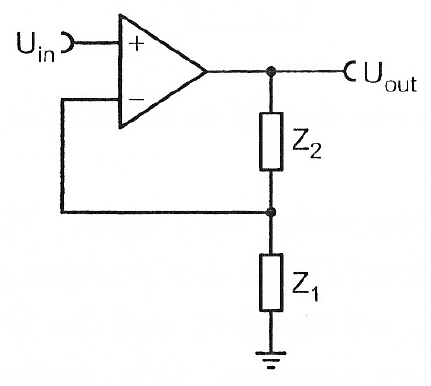
\includegraphics[width=.4\linewidth]{Anleitung/5_6-4.png}
	\caption{%
		\cite[Abbildung~5/6.4]{physik313-Anleitung}
	}
	\label{fig:5_6-4}
\end{figure}

In Abbildung~\ref{fig:5_6-4} ist die Schaltung eines nicht invertierenden
Verstärkers zu sehen. Die Verstärkung ist bei diesem:
\[
    v = \frac{\Uout}{\Uin} = \frac 1k = 1 + \frac{Z_2}{Z_1}
\]

\FloatBarrier
\subsubsection{Invertierender Verstärker}

\begin{figure}[htbp]
	\centering
	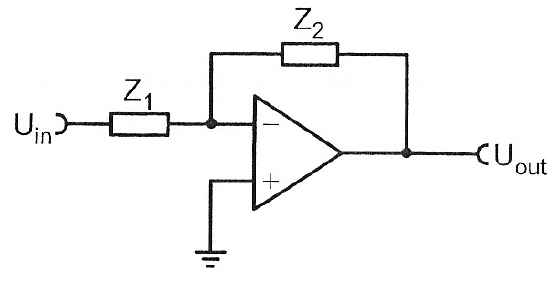
\includegraphics[width=.4\linewidth]{Anleitung/5_6-5.png}
	\caption{%
		\cite[Abbildung~5/6.5]{physik313-Anleitung}
	}
	\label{fig:5_6-5}
\end{figure}

Die Schaltung eines invertierenden Verstärkers ist in
Abbildung~\ref{fig:5_6-5} zu sehen. Die Verstärkung ist in diesem Fall:
\[
    v = -\frac{Z_2}{Z_1}
\]

\FloatBarrier
\subsubsection{Addierer}

Siehe Aufgabe~\ref{ssec:Aufgabe_F}.

\FloatBarrier
\subsubsection{Differenzverstärker}

In Abbildung~\ref{fig:5_6-7} ist die Schaltung eines Differenzverstärkers zu
sehen.

\begin{figure}[htbp]
	\centering
	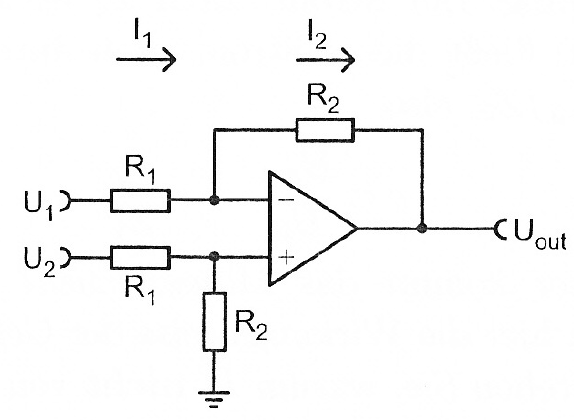
\includegraphics[width=.6\linewidth]{Anleitung/5_6-7.png}
	\caption{%
		\cite[Abbildung~5/6.7]{physik313-Anleitung}
	}
	\label{fig:5_6-7}
\end{figure}

Für die Verstärkung eines solchen Aufbaus, siehe Aufgabe~\ref{ssec:Aufgabe_G}.

\FloatBarrier
\subsubsection{Stromquelle}

Der Strom im rückkoppelnden Zweig in der Schaltung zum invertierenden
Verstärker (Abbildung~\ref{fig:5_6-5}) ist unabhängig vom Widerstand $Z_2$.
Dies liegt daran, dass der Strom, der durch $Z_1$ geht vollständig durch den
diesen Zweig fließen muss, da kein Strom in den Verstärker fließen kann. Damit
kann man die Schaltung für eine spannungsgesteuerte Stromquelle nutzen.


%%%%%%%%%%%%%%%%%%%%%%%%%%%%%%%%%%%%%%%%%%%%%%%%%%%%%%%%%%%%%%%%%%%%%%%%%%%%%%%
%                                  Aufgaben                                   %
%%%%%%%%%%%%%%%%%%%%%%%%%%%%%%%%%%%%%%%%%%%%%%%%%%%%%%%%%%%%%%%%%%%%%%%%%%%%%%%

\FloatBarrier
\section{Aufgaben}

\FloatBarrier
\subsection{Aufgabe A}

\begin{problem}
	Berechnen Sie $v$ für $k = \num{0.1}$, $v_0 = \num{e4}$ und $v_0 =
	\num{e5}$. Um wieviel Prozent weicht $v$ jeweils vom angestrebten Wert $1 /
	k$ ab?
\end{problem}

\begin{align*}
    v_\text{opt} &= \frac 1k = 10 \\
	v_{v_0 = 10^4} &= \frac 1{\num{0.1} + 10^{-4}} \approx \num{9.990} \\
	v_{v_0 = 10^5} &= \frac 1{\num{0.1} + 10^{-5}} \approx \num{9.999}
\end{align*}

Dies entspricht einer Abweichung von $\SI{0.1}\percent$ für $v_0 = \num{e4}$
und $\SI{.01}\percent$ für $v_0 = \num{e5}$.

\FloatBarrier
\subsection{Aufgabe B}

\begin{problem}
	Zeigen Sie, dass die Eingangsspannung des Verstärkers allgemein $U_x =
	\Uin / (1+kv_0)$ ist. Wie groß ist sie für den oben betrachteten Verstärker
	mit $k = \num{0.1}$, $v_0 = \num{e5}$, $\Uin = \SI 1{\volt}$?
\end{problem}

Es gilt
\begin{align*}
    U_x &= \Uin - k\Uout \\
        &= \Uin - kv_0U_x
    \intertext{Hieraus folgt}
    \Uin &= \del{1+kv_0}U_x
    \intertext{und daraus erhält man sofort die gesuchte Beziehung}
    U_x &= \frac {\Uin}{1+kv_0}
    \intertext{Für den oben betrachteten Verstärker ergibt sich}
    U_x &= \SI{e-4}{\volt}
\end{align*}

\FloatBarrier
\subsection{Aufgabe C}

\begin{problem}
    Berechnen Sie nun die Verstärkung eines Gleichtaktsignals (common mode
    signal, CM), also $\Delta U_+ = \Delta U_- = +\Delta \Uin$. Betrachten Sie
    dazu wieder die Änderung der Emitterspannungen und die daraus
    resultierenden Änderungen des Stromes durch $R_1$ (näherungsweise: $R_1 \gg
    \RE$). Zeigen Sie, dass $v_\text{CM} \approx -\RC / (2R_1)$. Wie ist die
    Gleichtaktunterdrückung einer solchen Schaltung für $\RE = \SI
    1{\kilo\ohm}$, $\RC = R_1 = \SI{100}{\kilo\ohm}$?
\end{problem}

Ändert man an beiden Eingängen die Spannung gleichermaßen um $+\Delta\Uin$,
hebt man auf beiden Seiten ebenfalls die Emitterspannungen um diesen Betrag.
Der zusätzliche Spannungsabfall an den Widerständen $\RE$ und $R_1$ findet
wegen $R_1 \gg \RE$ fast vollständig in $R_1$ statt. Der Strom, der dadurch
zusätzlich durch $R_1$ fließt, ist $\Delta I_1 = \Delta\Uin / R_1$. Die
Spannung, die über $\RC$ abfällt ändert sich dadurch um:
\[
    \Delta\UC = \RC\Delta\IC = \half\RC\Delta I_1 = \frac \RC {2R_1} \Delta\Uin
\]

$\Uout$ sinkt entsprechend um diesen Betrag.

Für die Gleichtaktverstärkung ergibt sich daher 
\[
    v_\text{CM} = \frac{\Uout}{\Uin} = -\frac \RC {2R_1}
\]

Die Gleichtaktunterdrückung ist dabei
\[
    \text{CMRR} = \frac {v_\text{CM}}{v_\text{diff}} = -\frac
    {\frac{\RC}{2R_1}}{\frac{\RC}{2\RE}} = -\frac{\RE}{R_1} = -0.01
\]

\FloatBarrier
\subsection{Aufgabe D}

\begin{problem}
    Betrachten Sie diese Schaltung (gemeint ist Schaltung~\ref{fig:5_6-4}) mit
    $Z_2 = R = \SI {100}{\kilo\ohm}$, $Z_1 = C = \SI {100}{\nano\farad}$. Wie
    ändert sich der Betrag von $Z_1$ mit der Frequenz und was bedeutet das für
    die Verstärkung? Was passiert für $f = 0$ und $f \to \infty$? Für welche
    Frequenz ist $\abs{Z_1} = R$? Berechnen Sie die Ausgangsspannung und
    daraus $v(f) = \abs{\Uout / \Uin}$, in dem Sie die komplexen Impedanzen für
    $R$ und $C$ benutzen. Stimmt Ihre obige Vorhersage für $v(0)$ und
    $v(\infty)$? Skizzieren Sie, wie $v(f)$ in einem Doppellogarithmischen Plot
    (Bode-Diagramm) aussieht!
\end{problem}

Da gilt $\abs{Z_1}=\frac 1{2\pi fC}$ ist, sinkt dieser mit steigender Frequenz
$f$. Für $f = 0$ gilt daher $\abs{Z_1} = \infty$, dadurch $v = 1$ und für $f
\to \infty$ gilt $\abs{Z_1} = 0$, dadurch $v \to \infty$.

Aus $R = \frac 1{2\pi fC}$ ergibt sich $f = \frac 1{2\pi RC} =
\SI{15.9}{\hertz}$.

Mit der gegebenen Beziehung erhält man

\[
    v = \abs{1 + \frac {Z_2}{Z_1}} = \abs{1 + \ii 2\pi RC f} = \sqrt{1 +
    4\pi^2R^2C^2 f^2} 
\]

Die Grenzwertbetrachtungen $f = 0$ und $f \to \infty$ ergeben das gleiche
Resultat, wie unsere obige Vermutung.

Eine Skizze der Abhängigkeit befindet sich in Abbildung~\ref{fig:5_6-D}.

\begin{figure}[htbp]
    \centering
    \includegraphics[width=\textwidth]{5_6-D.pdf}
    \caption{%
        Abhängigkeit der Verstärkung von der Frequenz
    }
    \label{fig:5_6-D}
\end{figure}

\FloatBarrier
\subsection{Aufgabe E}

\begin{problem}
	\[
		v = \frac\Uout\Uin = - \frac{Z_2}{Z_1}
	\]

	Woher kommt das Minuszeichen? Machen Sie sich auch hier die Wirkungsweise
	der Gegenkopplung klar! Verstehen Sie, warum $I_2$ \emph{nicht} von $Z_2$
	abhängt! Wie sind Eingangs- und Ausgangswiderstand dieser Schaltung?
\end{problem}

Der Strom $I_1$ wird durch die Potentialdifferenz zwischen Eingang und
virtueller Masse getrieben. Die Spannung ist $\Uin - 0$.

Der Strom muss durch $Z_2$ fließen, da die Eingänge des Operationsverstärkers
sehr hochohmig sind. Dazu muss der Operationsverstärker Arbeit leisten, in dem
er mit Hilfe seiner Versorgungsspannung die Spannung am Ausgang so hält, dass
der Strom $I_1$ auch durch $Z_2$ gezogen werden kann. Dazu erzeugt der
Operationsverstärker eine Potentialdifferenz von $0 - \Uout$. Die
Ausgangsspannung $\Uout$ wird festgelegt durch:
\[
	|\Uout| = I_2 Z_2 = I_1 Z_2
\]

Das Minuszeichen kommt daher, dass das Potential von Eingang zur virtuellen
Masse fällt, von der virtuellen Masse zum Ausgang jedoch weiter ins Negative
fällt. Es handelt sich ja um einen invertierenden Verstärker.

Die Gegenkopplung funktioniert so, dass einen kleine Erhöhung der
Eingangsspannung zu einem höheren Gradient im Widerstand $Z_1$ führt. Dadurch
wird mehr Strom $I_1$ angetrieben, der vom Operationsverstärker durch ein
ausreichend negatives Potential $\Uout$ durch $Z_2$ weiter getrieben wird.
Würde der Strom nicht weiter getrieben, so baut sich am invertierenden Eingang
eine positive Spannung auf, was den Operationsverstärker dazu bringt, mehr
negatives Potential an den Ausgang zu legen.

$I_2$ hängt nicht von $Z_2$ ab, da $I_1$ (mit der Betriebsspannung des
Operationsverstärkers) erzwungen wird. 

Der Eingangswiderstand ist:
\[
	\frac\Uin{I_1} = Z_1
\]

Der Ausgangswiderstand ist, nach den Formeln:
\[
	\frac\Uout{I_2} = - Z_2
\]

\subsection{Aufgabe F}
\label{ssec:Aufgabe_F}

\begin{problem}
	Zeigen Sie, dass die Schaltung in Abbildung~\ref{fig:5_6-6} die
	Eingangsspannungen folgendermaßen addiert:
	\[
		\Uout = c_1 U_1 + c_2 U_2 + \ldots + c_n U_n
		\quad \text{mit} \quad
		c_n = - \frac{R_0}{R_n}
	\]

	Berechnen Sie dazu wie oben die Ströme am invertierenden Eingang und
	benutzen Sie $U_+ = U_-$.
\end{problem}

\begin{figure}[htbp]
	\centering
	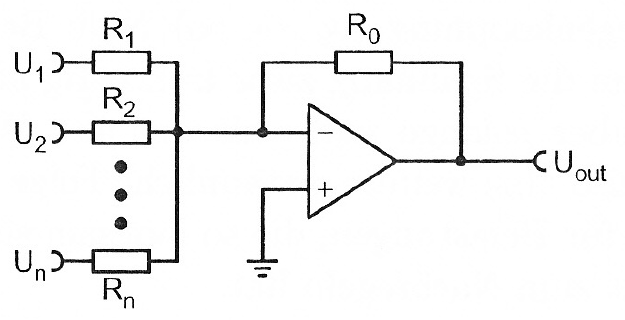
\includegraphics[width=.6\linewidth]{Anleitung/5_6-6.png}
	\caption{%
		\cite[Abbildung~5/6.6]{physik313-Anleitung}
	}
	\label{fig:5_6-6}
\end{figure}

Es herrscht ein Potentialgefälle $U_i - 0$ an jedem Widerstand. Die 0 ist
durch die Rückkopplung fix. Es fließen Ströme $I_i = U_i / R_i$.

Diese Ströme addieren sich auf, werden durch den Operationsverstärker durch den
Widerstand $R_0$ gezogen, wodurch ein Potential von
\[
	\Uout = - R_0 \sum_i \frac{U_i}{R_i}
\]
benötigt wird.

\subsection{Aufgabe G}
\label{ssec:Aufgabe_G}

\begin{problem}
	Erklären Sie die einzelnen Schritte und rechnen Sie das Endergebnis nach!
\end{problem}

Schritt:
\begin{equation}
	\label{eq:G1}
	U_+ = U_2 \frac{R_2}{R_1 + R_2}
\end{equation}

Dies ist ein unbelasteter Spannungsteiler von $U_2$ mit der Masse.

Schritt:
\begin{equation}
	\label{eq:G2}
	U_- = U_+
\end{equation}

Dies ist die Gleichgewichtseinstellung des Operationsverstärkers.

Schritt:
\begin{equation}
	\label{eq:G3}
	I_1 = \frac{U_1 - U_-}{R_1}
\end{equation}

$U_-$ ist das Potential am invertierenden Eingang. Die Potentialdifferenz
zwischen dem äußeren Eingang und dem Operationsverstärker zieht einen Strom
$I_1$ durch den Widerstand.

Schritt:
\begin{equation}
	\label{eq:G4}
	I_2 = I_1
\end{equation}

Operationsverstärker-Eingänge lassen keinen Strom zu. Daher wird der Strom
durch $R_2$ gezwungen.

Schritt:
\begin{equation}
	\label{eq:G5}
	I_2 = \frac{U_- - \Uout}{R_2}
\end{equation}

Umformen: $I_2 R_2$ erzeugt Potential $U_- - \Uout$.

\paragraph{Endergebnis}
\[
	\Uout = \frac{R_2}{R_1} \cdot (U_2 - U_1)
\]

Beginne mit \eqref{eq:G5}:
\begin{align*}
	I_2 &= \frac{U_- - \Uout}{R_2} \\
	R_2 I_2 &= U_- - \Uout \\
	\intertext{%
		Setze \eqref{eq:G2} für $U_-$ ein. Setze \eqref{eq:G1} für $U_+$ ein.
	}
	\Uout
	&= \del{1 + \frac{R_2}{R_1}} U_- - \frac{R_2}{R_1} U_1 \\
	&= \del{1 + \frac{R_2}{R_1}} U_2 \frac{R_2}{R_1 + R_2} - \frac{R_2}{R_1} U_1 \\
	&= \frac{R_1 + R_2}{R_1} U_2 \frac{R_2}{R_1 + R_2} - \frac{R_2}{R_1} U_1 \\
	&= \frac{R_2}{R_1} U_2 - \frac{R_2}{R_1} U_1 \\
	&= \frac{R_2}{R_1} \cdot (U_2 - U_1)
\end{align*}

\subsection{Aufgabe H}

\begin{problem}
	Erklären Sie, was bei einer konstanten negativen Eingangsspannung in der
	Schaltung und am Ausgang passiert.
\end{problem}

Der Eingang ist konstant negativ. Es fließt ein konstanter Strom $\Uin/R_1$.
Damit wird der Kondensator geladen. Die Spannung steigt. Bei konstanter $\Uin$
wird die Spannung von $C$ bis zur Betriebsspannung aufgeladen, dann kann
$\Uout$ nicht mehr positiv genug sein, um $C$ aufzuladen.

\subsection{Aufgabe I}

\begin{problem}
	Betrachten Sie die Schaltung als invertierenden Verstärker mit $Z_1 = R$.
	Bauen Sie für $Z_2$ einen Kondensator ein und berechnen Sie den
	Frequenzgang $v(\omega)$ und die Phasenbeziehung $\Phi(\omega)$ zwischen
	Ausgangs- und Eingangssignal.
\end{problem}

\begin{gather*}
	v = - \frac{Z_2}{Z_1} \\
	Z_1 = R \\
	Z_2 = \frac{1}{\ii \omega C} \\
	v = \ii \frac{1}{\omega RC}
\end{gather*}

Phase ist $\piup/2$, $v(\omega) = 1 / (\omega RC)$.

\subsection{Aufgabe J}

\begin{problem}
	Wie groß ist die zu erwartende maximale Schaltfrequenz für den im Praktikum
	verwendeten Operationsverstärker AD711 ($U_\text{max/min} = \pm
	\SI{14}\volt$)?
\end{problem}

Das sind \SI{28}{\volt} pro Schaltvorgang. Die slew rate ist mit
\SI{20}{\volt\per\milli\second} angegeben. Dies sind
\SI{2e7}{\volt\per\second}. Die zu erreichende Frequenz ist:
\[
	f = \frac{\SI{2e7}{\volt\per\second}}{\SI{28}\volt} = \SI{714}{\kilo\hertz}
\]

\FloatBarrier
\subsection{Aufgabe K}

\begin{problem}
	Skizzieren Sie den Spannungsverlauf am Ausgang und am Kondensator für $R_1
	= R_2$, $U_\text{max, min} = \pm \SI{14}\volt$. Durch welche Mathematische
	Funktion wird die Lade-/Entladekurve beschrieben?
\end{problem}

Da der Aufbau einen invertierenden Schmitt-Trigger enthält, ist der Ausgang
$\Uout$ mit einem Rechteck belegt. Der Kondensator wird mit einer konstanten
Spannung aufgeladen, die Ladekurve ist also exponentiell. Beides ist in
Abbildung~\ref{fig:K} skizziert.

\begin{figure}[htbp]
	\centering
	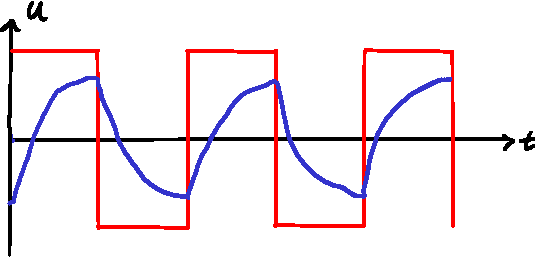
\includegraphics{K.pdf}
	\caption{%
		Spannungsverlauf. In rot die Spannung $\Uout$ am Ausgang des
		Operationsverstärkers. In blau die Spannung über dem Kondensator, die
		proportional zu seiner Ladung ist.
	}
	\label{fig:K}
\end{figure}

%%%%%%%%%%%%%%%%%%%%%%%%%%%%%%%%%%%%%%%%%%%%%%%%%%%%%%%%%%%%%%%%%%%%%%%%%%%%%%%
%                                Durchführung                                %
%%%%%%%%%%%%%%%%%%%%%%%%%%%%%%%%%%%%%%%%%%%%%%%%%%%%%%%%%%%%%%%%%%%%%%%%%%%%%%%

\FloatBarrier
\section{Durchführung – erster Versuchtstag}

\FloatBarrier
\subsection{Gruppeneinteilung für Versuch 6}

\FloatBarrier
\subsection{Nicht invertierender Verstärker}

Dadurch, dass wir eine Verstärkung $v$ einstellen, jedoch auch eine Verstärkung
$v$ messen, kommt es zum Benennungskonflikt. Daher wollen wir die
Soll-Verstärkung mit $V$ bezeichnen, während wir die gemessene Verstärkung aus
den Amplituden mit $v$ bezeichnen.

\subsubsection{Aufbau}

Wir bauen einen nicht invertierenden Verstärker auf, siehe
Abbildung~\ref{fig:5_6-4}. 

\subsubsection{Frequenzgang für $V = 11$}

Hier wählen wir die Widerstände so, dass eine Verstärkung von $V = 11$
eingestellt wird. In der Anleitung wird $R_1 = \SI{1}{\kilo\ohm}$ vorgegeben.

Die Verstärkung ist gegeben durch: \cite[Formel~5/6.6]{physik313-Anleitung}:
\[
	V = 1 + \frac{Z_2}{Z_1}
\]

Die zu erreichende Verstärkung von $V = 11$ mit $R_1 = \SI{1}{\kilo\ohm}$
erreichen wir, indem wir $R_2 = \SI{10}{\kilo\ohm}$ wählen.

Als Eingangssignal wählen wir ein Sinussignal mit \SI{100}{\milli\voltss}
Amplitude.

Um die Signalverstärkung $v$ direkt ablesen zu können, stellen wir Eingangs-
und Ausgangssignal gleichzeitig auf dem Oszillographen dar. Die Verstärkung am
Oszillographen wird so eingestellt, dass das Eingangssignal ein Kästchen groß
ist. Das Ausgangssignal wird auf die unterste Linie zentriert und gleich
skaliert.

Das Ablesen der Verstärkung $v$ beginnen wir bei der Transitfrequenz, um den
Abfall im Bode-Diagramm genauer als das Plateau vermessen zu können. Unsere
Messdaten sind in Tabelle~\ref{tab:Verstaerker-11}.

\begin{table}[htbp]
	\centering
	\begin{tabular}{SSS|S}
		{$f / \si\hertz$} &
		{$\Uin / \si\division$} &
		{$\Uout / \si\division$} &
		{$v$} \\
		\hline
		%< for f, uin, uout, v in table_verstaerker_11: >%
		<< f >> & << uin >> & << uout >> & << v >> \\
		%< endfor >%
	\end{tabular}
	\caption{%
		Messwerte für den Verstärker mit $V = 11$
	}
	\label{tab:Verstaerker-11}
\end{table}

Diese Daten sind in Abbildung~\ref{fig:Verstaerker-Bode} geplottet.

\begin{figure}[htbp]
	\centering
	\includegraphics[width=\linewidth]{Plot-Verstaerker.pdf}
	\caption{%
		Bode-Plot für den nicht invertierenden Verstärker
	}
	\label{fig:Verstaerker-Bode}
\end{figure}

Die Daten lassen wir mit Splines interpolieren. Dazu benutzen wir aus
SciPy\footnote{Version \texttt{python3-scipy-0.11.0+dfsg1-1ubuntu2}} die
eindimensionale Interpolation\footnote{\texttt{scipy.interpolate.interp1d}}.
Diese Splines sind im Plot als durchgezogene Linie eingezeichnet.

Von dieser Funktion lassen wir mit dem
Brent-Algorithmus\footnote{\texttt{scipy.optimize.brentq}} die Stelle finden,
bei der sie den Wert 1 hat. Die Frequenz ist dann die Transitfrequenz $\fT$.
Für die erste Messung erhalten wir eine Transitfrequenz von \SI{<< f_T_11
>>}{\hertz}.

Die Grenzfrequenz lassen wir ähnlich errechnen, dabei suchen wir die Frequenz,
bei der die Verstärkung von ihrem maximalen Wert auf $1/\sqrt2$ abgefallen ist.
Als maximalen Wert benutzen wir den maximalen Messwert. So erhalten wir hier
eine Grenzfrequenz von $f_\text{grenz} = \SI{<< f_grenz_11 >>}\hertz$.

Im Plot sind Transit- und Grenzfrequenz mit einer Raute bzw. einem Stern
markiert.

\subsubsection{Frequenzgang für $V = 101$}

Nun verändern wir die Widerstände so, dass $V = 101$. Dies erreichen wir mit
$R_2 = \SI{100}{\kilo\ohm}$. Wir fahren die Frequenzen so hoch, dass wir die
gemessenen Verstärkungen $v$ aus \numlist{80;60;40;20;10} abfahren. Unsere
Messwerte sind in Tabelle~\ref{tab:Verstaerker-101}.

\begin{table}[htbp]
	\centering
	\begin{tabular}{SSS|S}
		{$f / \si\hertz$} &
		{$\Uin / \si\division$} &
		{$\Uout / \si\division$} &
		{$v$} \\
		\hline
		%< for f, uin, uout, v in table_verstaerker_101: >%
		<< f >> & << uin >> & << uout >> & << v >> \\
		%< endfor >%
	\end{tabular}
	\caption{%
		Messwerte für den Verstärker mit $V = 101$
	}
	\label{tab:Verstaerker-101}
\end{table}

Diese Messpunkte tragen wir auch in das Diagramm
(Abbildung~\ref{fig:Verstaerker-Bode}) ein. Wir bestimmen die Transit- und
Grenzfrequenz. Die Transitfrequenz ist: $\fT = \SI{<< f_T_101 >>}{\hertz}$. Die
Grenzfrequenz ist: $f_\text{grenz} = \SI{<< f_grenz_101 >>}\hertz$.

\subsubsection{Frequenzgang für $V = 2$}

Da der Operationsverstärker die Verstärkung limitiert, und zwar auf 11, sollte
bei einer Soll-Verstärkung von $V = 2$ dies über eine deutlich größeren
Frequenzbereich möglich sein. Entsprechende Messwerte sind in
Tabelle~\ref{tab:Verstaerker-2} und Abbildung~\ref{fig:Verstaerker-Bode}.

\begin{table}[htbp]
	\centering
	\begin{tabular}{SSS|S}
		{$f / \si\hertz$} &
		{$\Uin / \si\division$} &
		{$\Uout / \si\division$} &
		{$v$} \\
		\hline
		%< for f, uin, uout, v in table_verstaerker_2: >%
		<< f >> & << uin >> & << uout >> & << v >> \\
		%< endfor >%
	\end{tabular}
	\caption{%
		Messwerte für den Verstärker mit $V = 2$
	}
	\label{tab:Verstaerker-2}
\end{table}

Für kleine Werte ist die Verstärkung $v = 2$. Für größere Frequenzen geht dies
in die restlichen Linien über.

Die Transitfrequenz ist: $\fT = \SI{<< f_T_2 >>}{\hertz}$. Die Grenzfrequenz
ist: $f_\text{grenz} = \SI{<< f_grenz_2 >>}\hertz$.

\subsubsection{Slew Rate mit $V = 101$}

In diesem Teil wählen wir als Eingangssignal ein Rechtecksignal mit einer
Frequenz von \SI{1}{\kilo\hertz}. Die Amplitude des Eingangssignals stellen wir
so ein, dass das Ausgangssignal eine Amplitude von \SI{20}{\voltss} hat.

An den Flanken des Ausgangssignals messen wir die slew rate, sie beträgt
\SI{2.2}{\division} bei einer Zeitauflösung
\SI{.5}{\micro\second\per\division}, also \SI{1.1}{\micro\second}.

Aus \cite[Tabelle~5/6.1]{physik313-Anleitung} ist ein Wert von
\SI{20}{\volt\per\micro\second} für den AD~711 zu erwarten, den wir auf unseren
Schaltbrettern haben.

Wir erhöhen die Frequenz, dabei achten wir auf die Ausgangsamplitude und
Signalform. Ab einer Frequenz von \SI{100}{\kilo\hertz} wird der Effekt sehr
deutlich. Das Ausgangssignal sieht Trapezförmig aus. Siehe
Abbildungen~\ref{fig:807} und \ref{fig:809}.

\begin{figure}[htbp]
	\centering
	\begin{minipage}{.45\linewidth}
		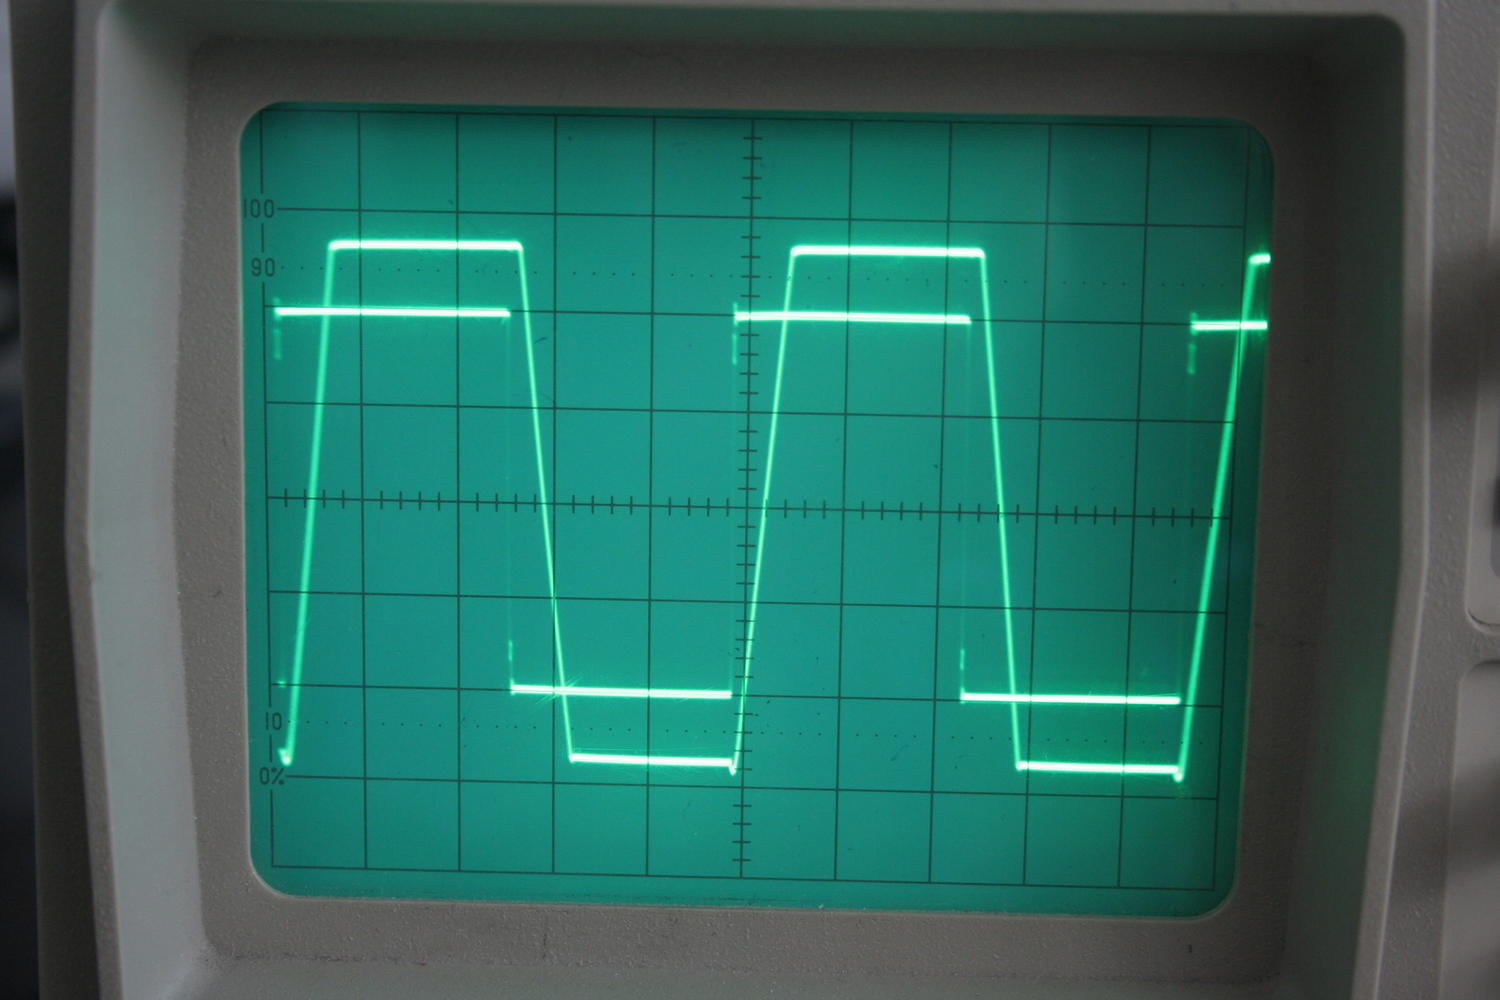
\includegraphics[width=\linewidth]{Oszi_Foto/5-807.jpg}
	\end{minipage}
	\hfill
	\begin{minipage}{.45\linewidth}
		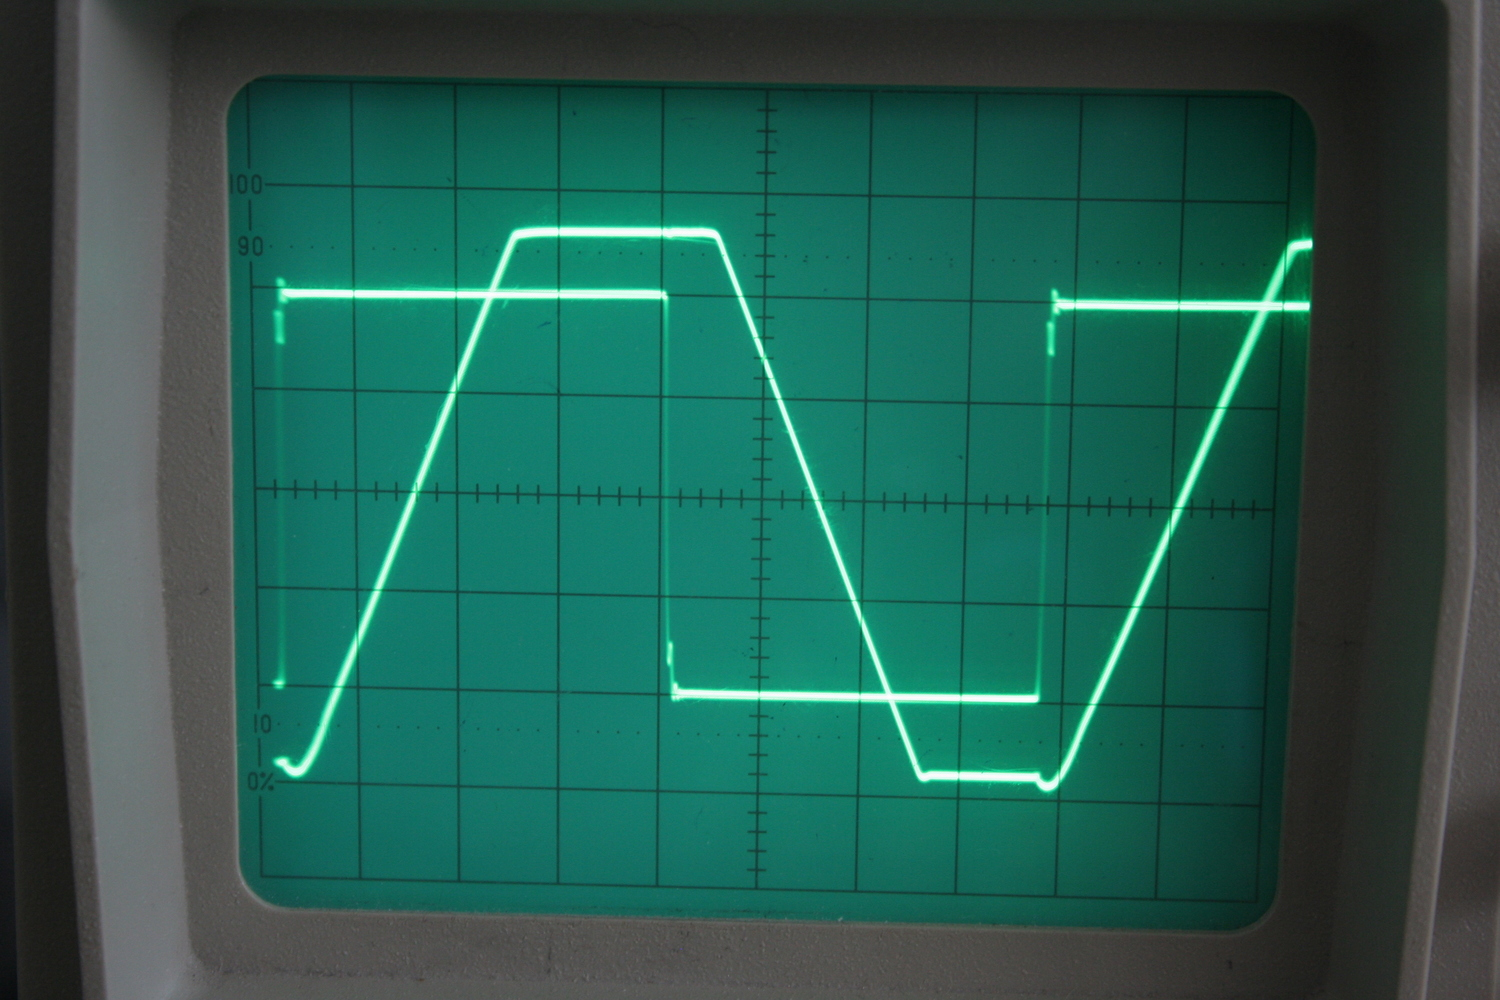
\includegraphics[width=\linewidth]{Oszi_Foto/5-808.jpg}
	\end{minipage}
	\caption{%
		Von links nach rechts: \SIlist{100;250}{\kilo\hertz}. Verstärkung
		\SIlist{.2;.5}{\micro\second\per\division}.
	}
	\label{fig:807}
\end{figure}

\begin{figure}[htbp]
	\centering
	\begin{minipage}{.45\linewidth}
		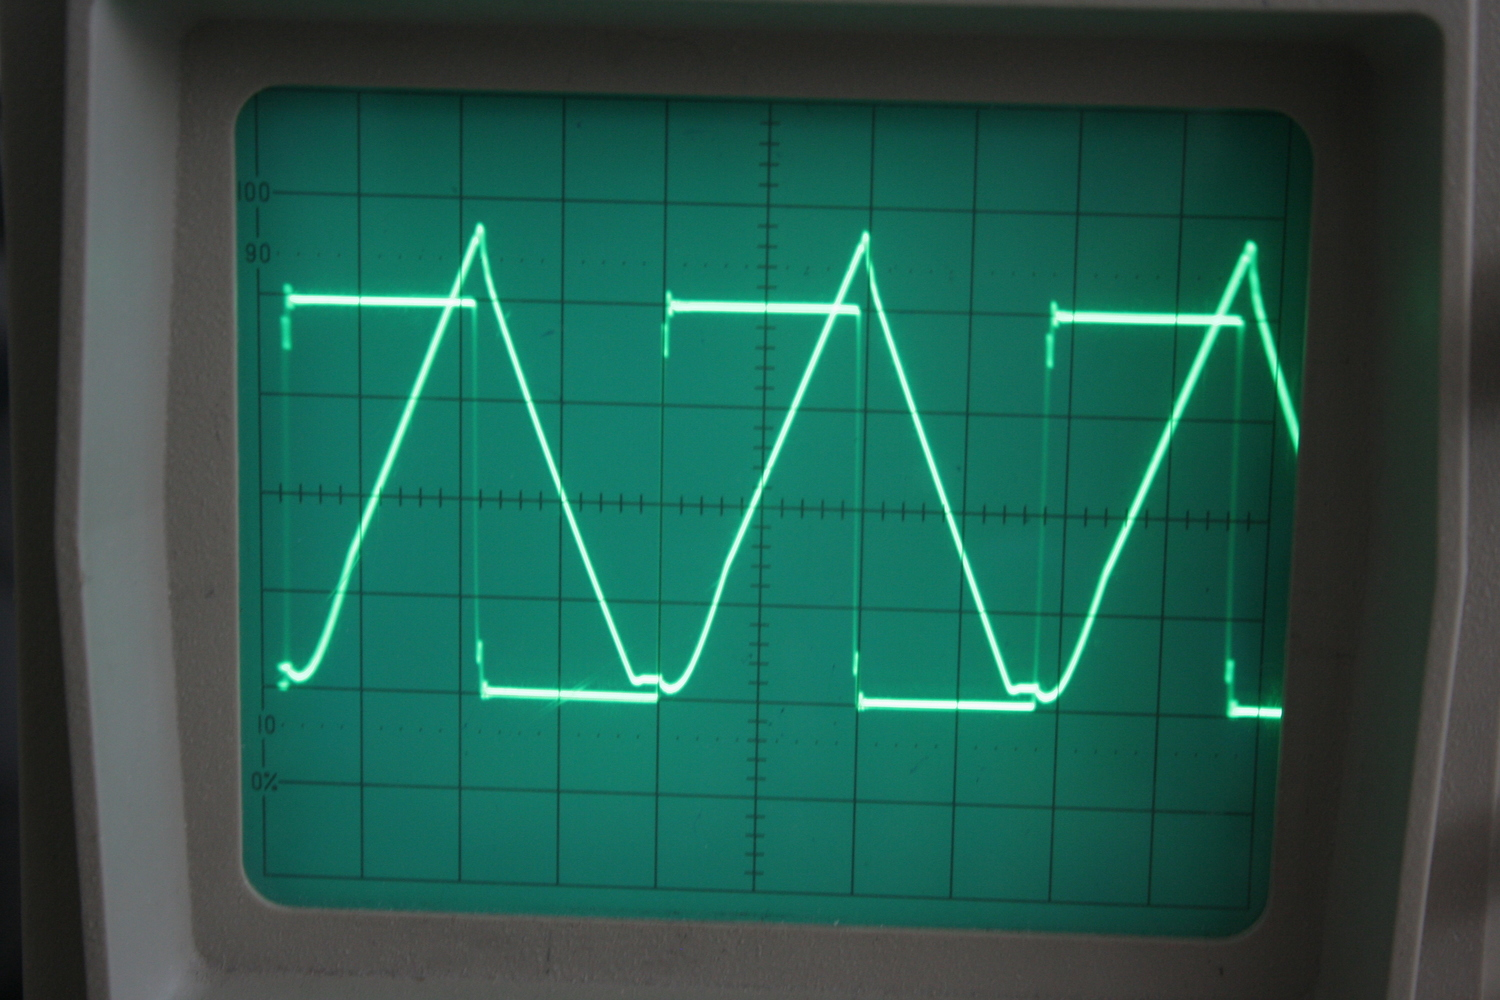
\includegraphics[width=\linewidth]{Oszi_Foto/5-809.jpg}
	\end{minipage}
	\hfill
	\begin{minipage}{.45\linewidth}
		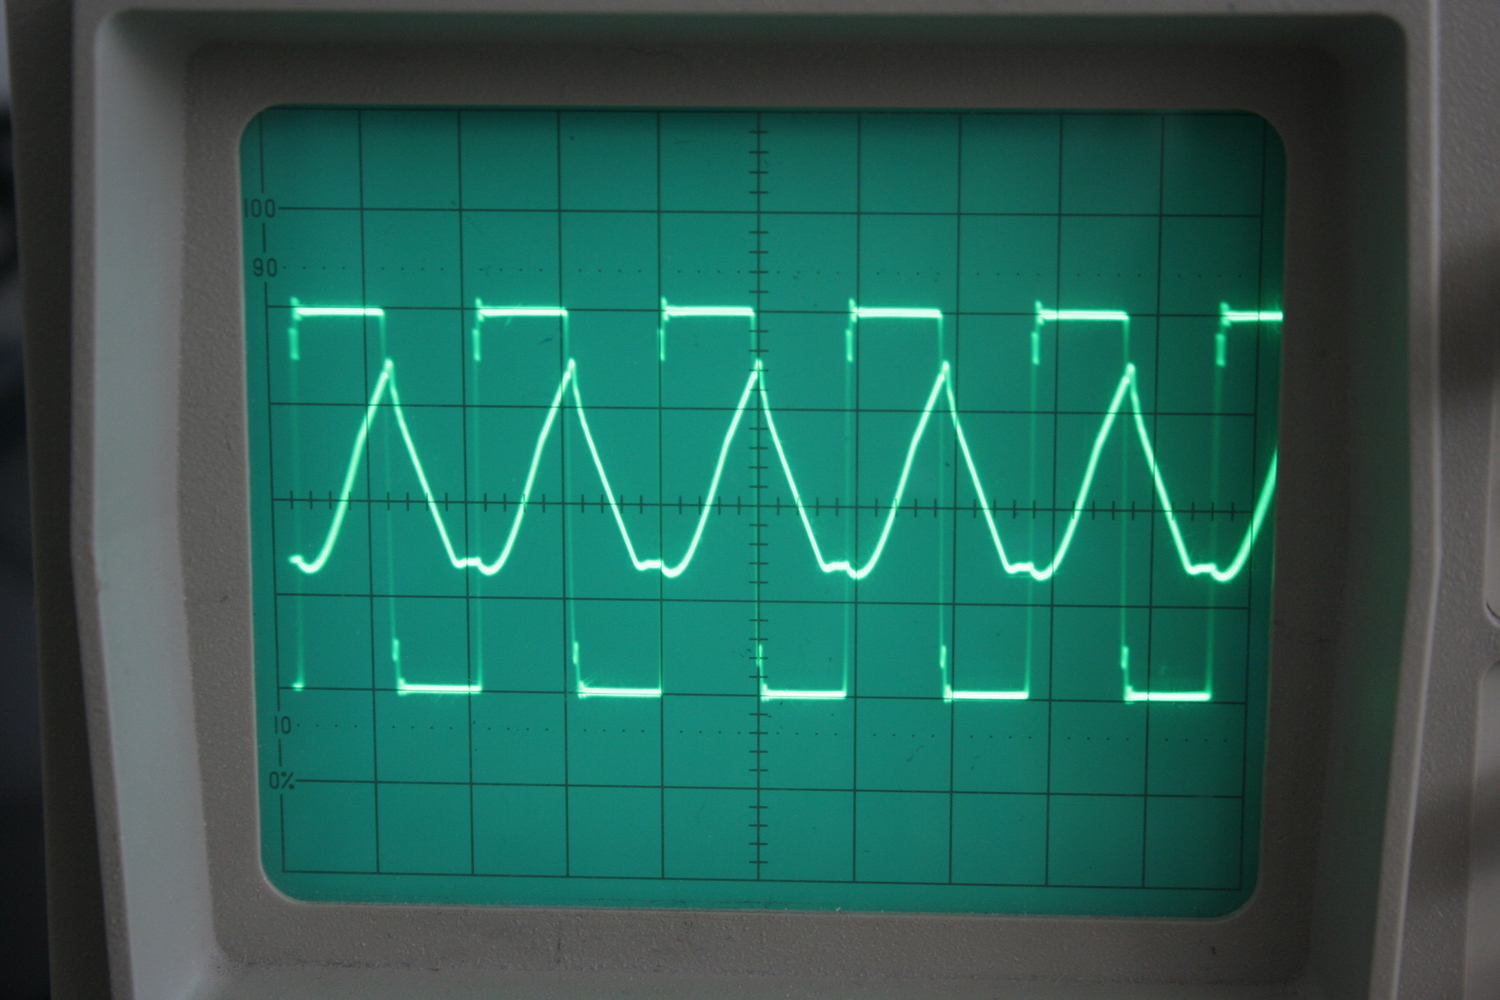
\includegraphics[width=\linewidth]{Oszi_Foto/5-810.jpg}
	\end{minipage}
	\caption{%
		Von links nach rechts: \SIlist{500;1000}{\kilo\hertz}. Verstärkung
		\SI{.5}{\micro\second\per\division}.
	}
	\label{fig:809}
\end{figure}

Nun schalten wir auf ein Sinussignal und vergleichen mit dem Rechtecksignal.

Bei einem Sinussignal sieht das Ausgangssignal genauso aus wie beim
Rechtecksignal. Wir glauben, dass das daran liegt, dass bei einem
Eingangssignal von \SI{20}{\volt} die Betriebsspannung des
Operationsverstärkers sehr schnell an ihr Maximum kommt.

\subsubsection{Kapazität in Serie mit $V = 11$}

Zuletzt stellen wir $V = 11$ ein, in dem wir die in der Aufgabenstellung
angegebenen Werte für die Widerstände benutzen: $R_1 = \SI{10}{\kilo\ohm}$ und
$R_2 = \SI{100}{\kilo\ohm}$. Außerdem schalten wir eine Kapazität von
\SI{.1}{\micro\farad} in Serie mit $R_1$.

Theoretisch erwarten wir, dass $Z_1 = R_1 + 1/(\ii \omega C)$ für kleine
Frequenzen groß, für große jedoch bis auf $R_1$ klein wird. Die Verstärkung war
mit gegeben als:
\[
	V = 1 + \frac{Z_2}{Z_1}
\]

Damit wird gilt für die Verstärkung:
\[
	\lim_{f \to 0} V = 1
	\eqnsep
	\lim_{f \to \infty} V = 1 + \frac{R_2}{R_1}
\]

Der Kondensator sollte sich bei einer Frequenz von $1/(\omega C) = R_1$
bemerkbar machen. Dies ist:
\[
	\omega = \frac1{R_1 C} = \SI{1000}{\radian\per\second} = \SI{6200}\hertz
\]

Wir messen für einige Frequenzen die Verstärkung. Die Messwerte sind in
Tabelle~\ref{tab:Verstaerker-c} und in Abbildung~\ref{fig:Verstaerker-Bode}.

\begin{table}[htbp]
	\centering
	\begin{tabular}{SSS|S}
		{$f / \si\hertz$} &
		{$\Uin / \si\division$} &
		{$\Uout / \si\division$} &
		{$v$} \\
		\hline
		%< for f, uin, uout, v in table_verstaerker_c: >%
		<< f >> & << uin >> & << uout >> & << v >> \\
		%< endfor >%
	\end{tabular}
	\caption{%
		Messwerte für den Verstärker mit $V = 11$ und einer Kapazität von
		\SI{.1}{\micro\farad} in Serie
	}
	\label{tab:Verstaerker-c}
\end{table}

Die Transitfrequenz ist: $\fT = \SI{<< f_T_c >>}{\hertz}$ Die Grenzfrequenz
ist: $f_\text{grenz} = \SI{<< f_grenz_c >>}\hertz$.

Die Grenzen für große und kleine Frequenzen stimmen überein. Der Kondensator
hat wirklich einen Einfluss ab der berechneten Frequenz.

\FloatBarrier
\subsubsection{Zusammenfassung}

\begin{table}[htbp]
	\centering
	\begin{tabular}{lSS}
		{Aufbau} &
		{$\fT / \si\hertz$} &
		{$f_\text{grenz} / \si\hertz$} \\
		\hline
		$V = 11$ & << f_T_11 >> & << f_grenz_11 >> \\
		$V = 101$ & << f_T_101 >> & << f_grenz_101 >> \\
		$V = 2$ & << f_T_2 >> & << f_grenz_2 >> \\
		$V = 11$ mit $C$ & << f_T_c >> & << f_grenz_c >> \\
	\end{tabular}
	\caption{%
		Zusammenfassung der charakteristischen Frequenzen
	}
	\label{tab:Verstaerker-Zusammenfassung}
\end{table}

\FloatBarrier
\subsection{Addierer}

Wir bauen einen Addierer mit drei Eingängen auf, wie in
Abbildung~\ref{fig:5_6-6} schematisch dargestellt. Als Eingangsquelle benutzen
dir den Dreifachsinusgenerator. Dieser liefert die Frequenzen
\SIlist{50;100;150;200}{\hertz}. Da wir für die Fourierreihe des Sägezahns
(Abbildung~\ref{fig:saegezahn}) ganzzahlige, aufeinanderfolgende Vielfache
brauchen, benutzen wir die Eingänge mit \SIlist{50;100;150}{\hertz}. Die
Amplituden wählen wir relativ $1$, $1/2$ und $1/3$. Daraus ergibt sich ein
Sägezahn, der allerdings noch deutlich runde Ecken hat.

Unser Ergebnis ist in Abbildung~\ref{fig:811} zu sehen.

\begin{figure}[htbp]
	\centering
	\includegraphics[width=\linewidth]{Plot-Saegezahn.pdf}
	\caption{%
		Darstellung des Sägezahns in Fourierkomponenten.
	}
	\label{fig:saegezahn}
\end{figure}

Den Sägezahn, den wir erreicht haben, ist in Abbildung~\ref{fig:811}.

\begin{figure}[htbp]
	\centering
	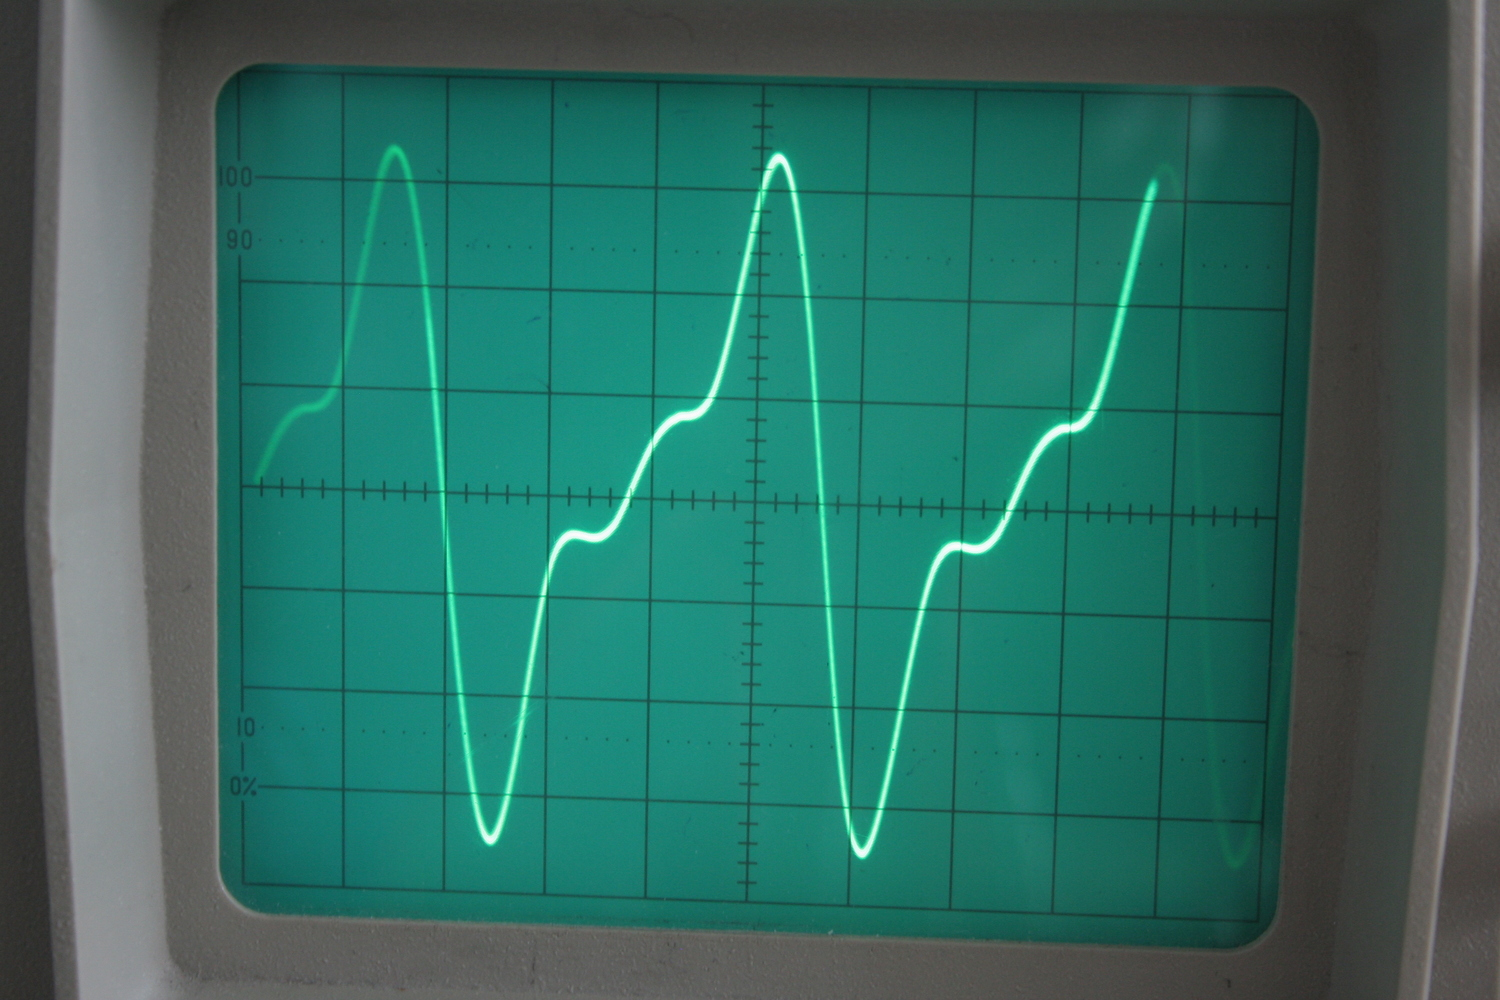
\includegraphics[width=.45\linewidth]{Oszi_Foto/5-811.jpg}
	\caption{%
        Sägezahn aus drei überlagerten Sinuskurven.
	}
	\label{fig:811}
\end{figure}

\FloatBarrier
\subsection{Konstantstromquelle}

\subsubsection{Aufbau}

Wir bauen die Konstantstromquelle aus Abbildung~\ref{fig:5-1} auf. Dabei sind
$R_1 = \SI{47}{\kilo\ohm}$ und $R_2 = \SI{10}{\kilo\ohm}$ in der Anleitung
vorgegeben.

\begin{figure}[htbp]
	\centering
	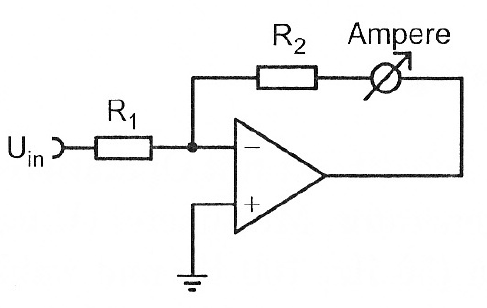
\includegraphics[width=.5\linewidth]{Anleitung/5-1.png}
	\caption{%
		\cite[Abbildung~5.1]{physik313-Anleitung}
	}
	\label{fig:5-1}
\end{figure}

\subsubsection{Strom durch Rückkopplungszweig}

Bei einer Eingangsspannung von \SI{9.4}{\volt} sollte der Strom im
Rückkopplungszweig ($I_2$) der Strom sein, der auch durch $R_1$ fließt. Also:
\[
	I_2
	= I_1
	= \frac\Uin{R_1}
	= \frac{\SI{9.4}\volt}{\SI{47}{\kilo\ohm}}
	= \SI{200}{\micro\ampere}
\]

Wir messen mit einem Digitalmultimeter nach und erhalten
\SI{.195}{\milli\ampere}. Die Abweichung ist mit der Ungenauigkeit der
angelegten Spannung zu erklären.

\subsubsection{Variable Last}

$R_2$ wird durch ein Potentiometer ersetzt. Wir variieren $R_2$ und beobachten
den Strom. Zu erwarten ist, dass der Strom konstant bleibt, da der
Operationsverstärker die Ausgangsspannung so regelt, dass der Strom durch $R_2$
konstant bleibt. Dies konnten wir mit unserer Messung bestätigen. Wenn die
benötigte Spannung über die Versorgungsspannung geht,
kann der Operationsverstärker jedoch nicht mehr weiter regeln, der Strom nimmt
ab.

Dies widerspricht nicht dem Ohm'schen Gesetz, im Gegenteil. Die Spannung wird
vom Operationsverstärker so verändert, dass $I = U/R$ konstant bleibt. Es ist
also die Spannung, die sich ändert. Die können wir Prüfen, indem wir mit einem
Multimeter über dem Widerstand abgreifen, oder direkt $\Uout$ zwischen Ausgang
und Masse abgreifen.

Die Spannung über dem Potentiometer variiert im Bereich
\SIrange{0}{8.85}{\volt}.

\subsubsection{Halbieren des Stroms}

Der Strom kann halbiert werden, indem die Eingangsspannung halbiert wird, oder
$R_1$ verdoppelt wird.

\FloatBarrier
\subsection{Integrator}

\subsubsection{Aufbau}

Wir bauen einen Integrator nach Abbildung~\ref{fig:5_6-11} auf. Die
Dimensionierung ist mit $C = \SI{100}{\nano\farad}$ und $R = \SI1{\mega\ohm}$
vorgegeben. Der Eingang wird mit einem symmetrischen Rechtecksignal mit
\SI{100}{\hertz} und \SI{1}{\voltss} belegt.

\begin{figure}[htbp]
	\centering
	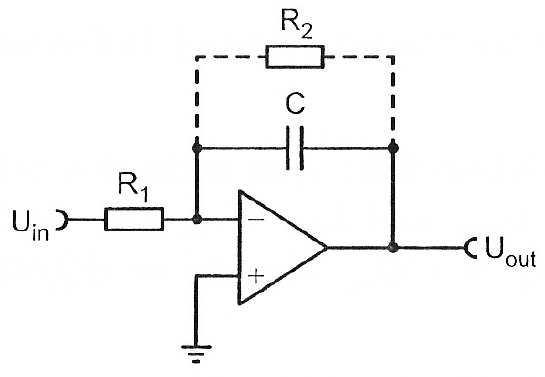
\includegraphics[width=.5\linewidth]{Anleitung/5_6-11.png}
	\caption{%
		\cite[Abbildung~5/6.11]{physik313-Anleitung}
	}
	\label{fig:5_6-11}
\end{figure}

Auf dem Oszillographen beobachten wir Ein- und Ausgang gleichzeitig.

\begin{figure}[htbp]
	\centering
	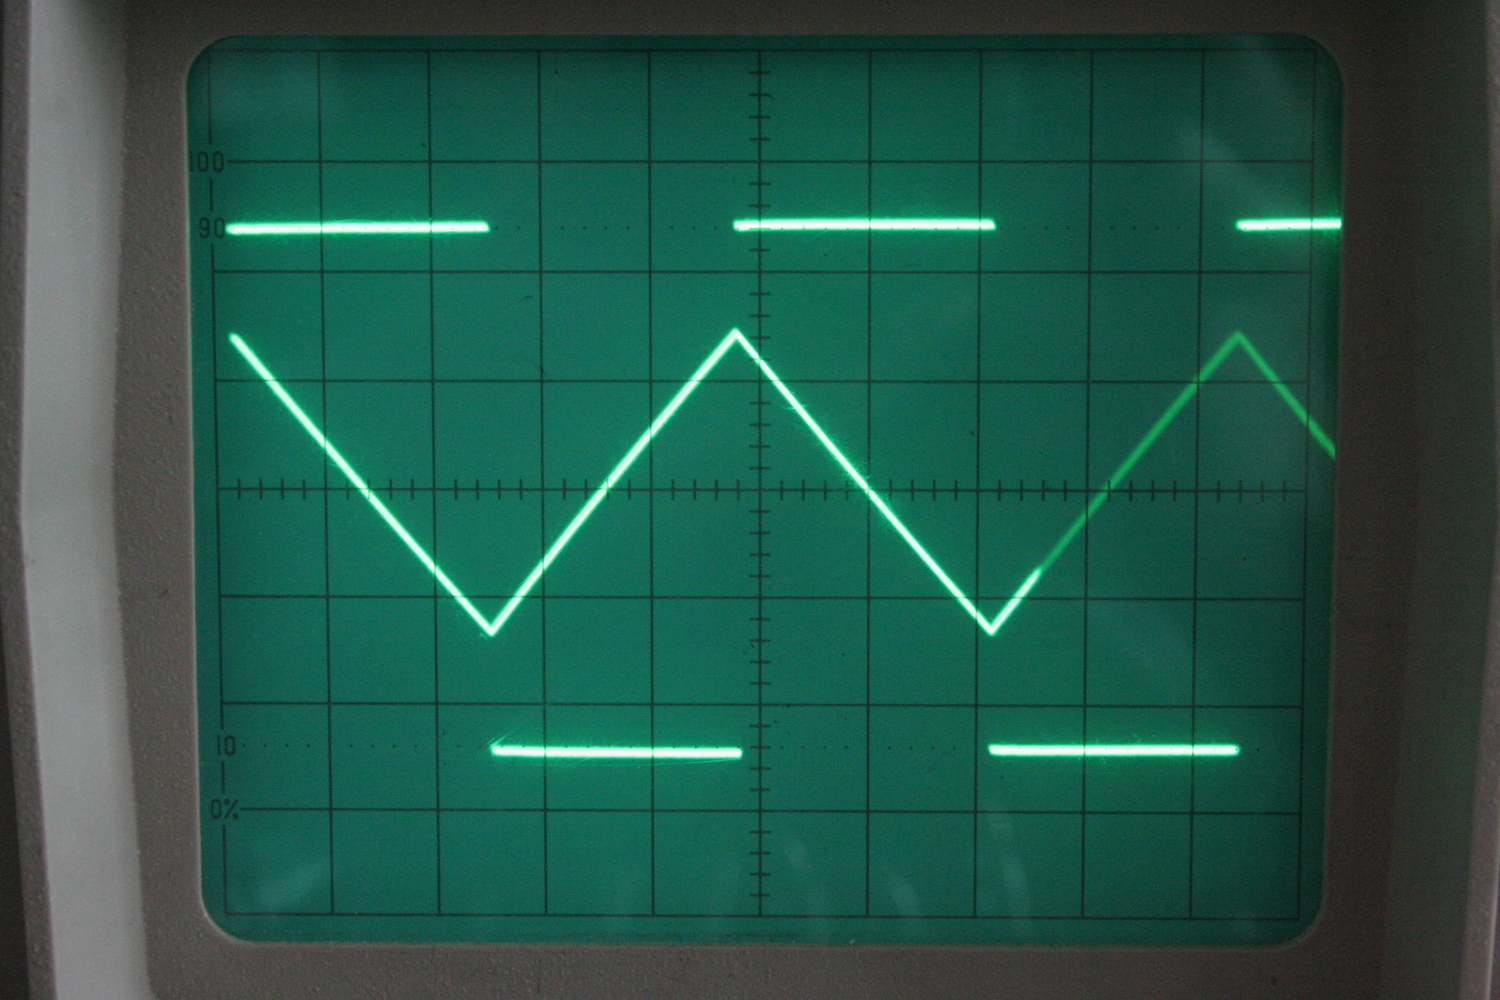
\includegraphics[width=.45\linewidth]{Oszi_Foto/5-813.jpg}
	\caption{%
		Verstärkung \SI{.2}{\volt\per\division}. Zeitbasis
		\SI{2}{\milli\second\per\division}.
	}
	\label{fig:813}
\end{figure}

Dabei sehen wir, dass der Kondensator mit einem konstanten Strom auf- und
entladen wird. Dadurch wird die Ladekurve gerade, siehe
Abbildung~\ref{fig:813}.

\subsubsection{Verschiedene Eingangswerte}

Wir verändern die Eingangsfrequenz- und Spannung und beobachten.

Die Eingangsamplitude ist proportional zur Maximalladung des Kondensators. Bei
verschiedenen Frequenzen bleibt die Steigung der Ladekurve konstant, da ja der
Strom gleich bleibt. Bei einer höheren Frequenz ist die Ladezeit jedoch
geringer, so dass die Maximalladung geringer wird.

\subsubsection{Weglassen von $R_2$}

In der Anleitung steht nun:

\begin{quote}
	Was geschieht, wenn Sie $R_2$ weglassen?
\end{quote}

Davor stand jedoch:

\begin{quote}
	Ersetzen Sie in Abbildung~\ref{fig:5-1} den Widerstand $R_2$ und das
	Amperemeter durch eine Parallelschaltung von $C$ […] und $R$ […].
\end{quote}

Somit ist der Widerstand $R_2$ bereits nicht mehr vorhanden.

\subsubsection{Sinussignal auf den Eingang}

Wie geben ein Sinussignal auf den Eingang und betrachten die Phasenverschiebung
zwischen Ein- und Ausgang.

Der Ausgang ist um $\piup/2$ voraus.

Nun schalten wir den Oszillographen in den XY-Betrieb und beobachten
Lissajous-Figuren. Da die Frequenzen gleich sind und es nur eine
Phasenverschiebung gibt, sind es Ellipsen, siehe Abbildung~\ref{fig:814}.

\begin{figure}[htbp]
	\centering
	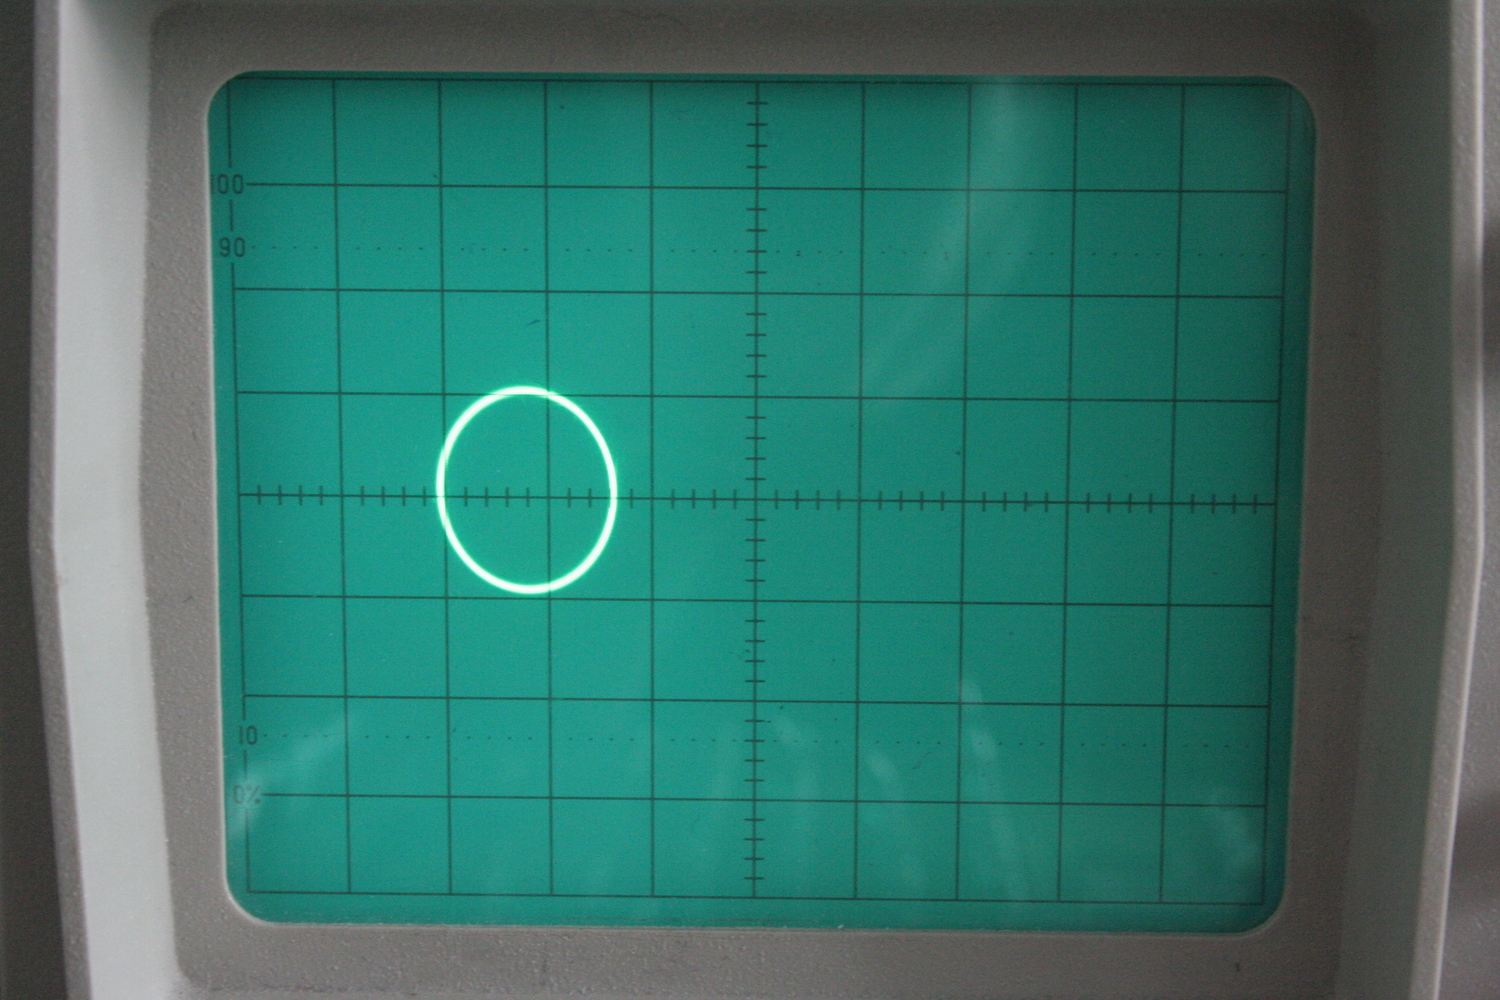
\includegraphics[width=.45\linewidth]{Oszi_Foto/5-814.jpg}
	\caption{%
		Verstärkung \SIlist{.5;.2}{\volt\per\division}. \SI{100}{\hertz}.
		XY-Modus.
	}
	\label{fig:814}
\end{figure}

\FloatBarrier
\subsection{Differenzverstärker}

\subsubsection{Aufbau}

Gemäß Abbildung~\ref{fig:5_6-7} bauen wir einen Differenzverstärker auf.

\subsubsection{Funktionsüberprüfung}

Wir überprüfen die Funktion mit einem Sinussignal auf dem einen Eingang und
einer Gleichspannung auf dem anderen Eingang. Die Gleichspannung wird von uns
variiert. Zuletzt vertauschen wir die Eingänge.

Mit der Spannungseinstellung am Netzteil können wir in der Tat die Höhe des
Ausgangssignal verschieben.

\subsubsection{Schwebung}

Mit Hilfe des separaten Sinusgenerators, den wir bereits beim Addierer benutzt
haben, und dem variablen Funktionsgenerator erzeugen wir eine Schwebung.

Es kommt zu einer Schwebung. Um dies gut sichtbar zu machen, haben wir ein
kleines Video bereitgestellt:

\url{http://chaos.stw-bonn.de/users/mu/uploads/2013-09-02/Schwebung.mp4} (6~MB)

\FloatBarrier
\subsection{Freiwillige Aufgabe}

Die freiwillige Aufgabe (Abbildung~\ref{fig:5-2}) lassen wir aus.

\begin{figure}[htbp]
	\centering
	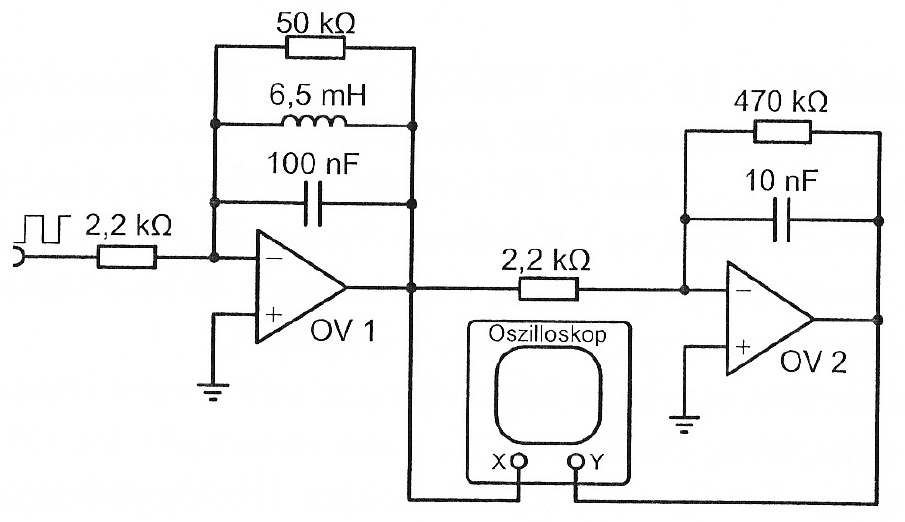
\includegraphics[width=.8\linewidth]{Anleitung/5-2.png}
	\caption{%
		\cite[Abbildung~5.2]{physik313-Anleitung}
	}
	\label{fig:5-2}
\end{figure}

%%%%%%%%%%%%%%%%%%%%%%%%%%%%%%%%%%%%%%%%%%%%%%%%%%%%%%%%%%%%%%%%%%%%%%%%%%%%%%%
%                                Durchführung                                %
%%%%%%%%%%%%%%%%%%%%%%%%%%%%%%%%%%%%%%%%%%%%%%%%%%%%%%%%%%%%%%%%%%%%%%%%%%%%%%%

\FloatBarrier
\section{Durchführung – zweiter Versuchstag}

%%%%%%%%%%%%%%%%%%%%%%%%%%%%%%%%%%%%%%%%%%%%%%%%%%%%%%%%%%%%%%%%%%%%%%%%%%%%%%%
%                                  Literatur                                  %
%%%%%%%%%%%%%%%%%%%%%%%%%%%%%%%%%%%%%%%%%%%%%%%%%%%%%%%%%%%%%%%%%%%%%%%%%%%%%%%

\FloatBarrier
\IfFileExists{\bibliographyfile}{
	\bibliography{\bibliographyfile}
}{}

\end{document}

% vim: spell spelllang=de tw=79
